% !TEX TS-program = xelatex
% !TEX encoding = UTF-8
\documentclass{article}

\usepackage{amsmath,amssymb,amsfonts}
\usepackage{graphicx}
\usepackage{xcolor}
\usepackage{geometry}
\geometry{top = 1.5 cm, bottom = 1.5 cm}


\title{Revisit to the theoretical analysis of a classical piezoelectric cantilever energy harvester}
\author{Maoying Zhou}
\date{\today}

\begin{document}

\maketitle


\section{Introduction}

The soaring depletion of fossil fuels and the growing awareness of environmental protection renders the challenge of renewable and sustainable energy sources for scientists and engineers. Apart from nuclear energy, wind energy, and solar energy, ambient energy harvesting has been proposed as an alternative to batteries for more than twenty years. Numerous principles, mechanisms, implementations, and applications have been put forward to deepen the understanding of energy harvesting, to find the routine for the development of new devices, to apply the devices to new situations. Among all these devices, piezoelectric energy harvesting devices have attracted much attention due to their simplicity of structure and superiority of performance. 

Generally a piezoelectric energy harvesting device consists of some piezoelectric elements and some vibration transduction structure for the hosting of these elements. A key problem in the research of piezoelectric element based energy harvesting is to improve the output of those devices. A key point is to understand the mechanics and coupling behind the devices.


\section{Outline of the paper}
The outline of the paper should be as follows:
\begin{itemize}
    \item To obtain the closed form solution of the CPEH problem using the harmonic balance method
    \item Analyze the dependence of relative displacement function $u(z;\delta)$
    \item Tackling the dependence of output index $\chi_p$ and output measures $\tilde{V}_p$, $\tilde{I}_p$, and $\tilde{P}_p$ upon the electromechanical coupling factor $\delta$ and base excitation frequency $f_b$
    \item Derive the asymptotic expansion of the CPEH problem for the displacement function $u(z;\delta)$ and the output index $\chi_p$
    \item Explore the approximation error of the asymptotic expansion and provide some clues to improve the performance
\end{itemize}




\section{Summary of the interested equations}

The dynamic equations for a typical piezoelectric composite cantilever beam is 
\begin{equation}
    B_p \frac{\partial^4 w(x,t)}{\partial x^4} + m_p \frac{\partial^2 w(x,t)}{\partial t^2} = 0,
\end{equation}
where $B_p$ is the equivalent bending stiffness and $m_p$ is the line mass density of the piezoelectric cantilever beam. If the piezoelectric elements attached to the cantilever beam is connected to an external electrical load $R_l$, we have 
\begin{equation}
    \frac{d Q_p(t)}{d t} + \frac{V_p(t)}{R_l} = 0.
\end{equation}
For the underlying physics, we have the following constitutive equations
\begin{equation}
    \begin{aligned}
        M_p(x,t) &= B_p \frac{\partial^2 w(x,t)}{\partial x^2} - e_p V_p(t), \\
        q_p(x,t) &= e_p \frac{\partial^2 w(x,t)}{\partial x^2} + \varepsilon_p V_p(t),
    \end{aligned}
\end{equation}
or equivalently,
\begin{equation}
    \left\{\begin{aligned}
        M_p(x,t) &= B_p \frac{\partial^2 w(x,t)}{\partial x^2} - e_p V_p(t), \\
        Q_p(x,t) &= e_p \left.\left[ \frac{\partial w(x,t)}{\partial x} \right]\right|_0^{l_p} + C_p V_p(t).
    \end{aligned}\right.
\end{equation}

One end of the cantilever beam is fixed while the other end is free. So the boundary conditions are
\begin{equation}
    \left\{\begin{aligned}
        w(0,t) &= w_b(t), \\
        \frac{\partial w(0,t)}{\partial x} &= 0,
    \end{aligned}\right.
\end{equation}
and
\begin{equation}
    \left\{\begin{aligned}
        M_p(l_p,t) &= B_p \frac{\partial^2 w(l_p,t)}{\partial x^2} - e_p V_p(t) = 0, \\
        N_p(l_p,t) &= \frac{\partial M_p(l_p,t)}{\partial x} = B_p \frac{\partial^3 w(l_p,t)}{\partial x^3} = 0.
    \end{aligned}\right.
\end{equation}


\section{Theoretical solution to the problem}

In the classical energy harvesting applications, the cantilever beam is subject to a periodical base excitation $w_b(t)$. Thus the dynamic response of the cantilever beam is decomposed as 
\begin{equation}
    w(x,t) = w_b(t) + w_{rel}(x,t),
\end{equation}
where $w_{rel}(x,t)$ is the relative displacement function of the cantilever beam. In this way, the system is converted into 
\begin{equation}
    B_p \frac{\partial^4 w_{rel}(x,t)}{\partial x^4} + m_p \frac{\partial^2 w_{rel}(x,t)}{\partial t^2} = - m_p \frac{\partial^2 w_{b}(t)}{\partial t^2},
\end{equation}
\begin{equation}
    e_p \left.\left[ \frac{\partial^2 w_{rel}(x,t)}{\partial x \partial t}\right]\right|_0^{l_p} + C_p \frac{d V_p(t)}{d t} + \frac{V_p(t)}{R_l} = 0.
\end{equation}
\begin{equation}
    \left\{\begin{aligned}
        w_{rel}(0,t) &= 0, \\
        \frac{\partial w_{rel}(0,t)}{\partial x} &= 0,
    \end{aligned}\right.
\end{equation}
and
\begin{equation}
    \left\{\begin{aligned}
        B_p \frac{\partial^2 w_{rel}(l_p,t)}{\partial x^2} - e_p V_p(t) &= 0, \\
        \frac{\partial^3 w_{rel}(l_p,t)}{\partial x^3} &= 0.
    \end{aligned}\right.
\end{equation}

Considering a sinusoidal base excitation
\begin{equation}
    w_b(t) = \eta_b e^{j \sigma_b t}
\end{equation}
where $\xi_b$ is usually a real vibration amplitude, the steady state solution for the above system can be reasonably set as
\begin{equation}
    w_{rel}(x,t) = \eta_{rel}(x) e^{j \sigma_b t},\quad V_p(t) = \tilde{V}_p e^{j \sigma_b t},
\end{equation}
where $\eta_{rel}(x)$ and $\tilde{V}_p$ are complex amplitudes. Then the above system is again simplified as 
\begin{equation}
    B_p \frac{\partial^4 \eta_{rel}(x)}{\partial x^4} - m_p \sigma_b^2 \eta_{rel}(x) = m_p \sigma_b^2 \eta_{b},
\end{equation}
\begin{equation}
    \left\{\begin{aligned}
        \eta_{rel}(0) &= 0, \\
        \frac{\partial \eta_{rel}(0)}{\partial x} &= 0,
    \end{aligned}\right.
\end{equation}
and
\begin{equation}
    \left\{\begin{aligned}
        B_p \frac{\partial^2 \eta_{rel}(l_p)}{\partial x^2} + \frac{j \sigma_b R_l }{1 + j \sigma_b C_p R_l } e_p^2 \frac{\partial \eta_{rel}(l_p)}{\partial x} &= 0, \\
        \frac{\partial^3 \eta_{rel}(l_p)}{\partial x^3} &= 0.
    \end{aligned}\right.
\end{equation}
\textcolor{red}{Note that here we assume a sinusoidal steady state response, which is not actually validated theoretically. }


Obviously we can have the following dimensionless scheme:
\begin{equation}
    \eta_{rel} \sim u \eta_b ,\quad x \sim z l_p 
\end{equation}
and therefore the following dimensionless parameters
\begin{equation}
    \sigma = \sigma_b \sqrt{\frac{m_p l_p^4}{B_p}}, \quad \beta = R_l C_p \sqrt{\frac{B_p}{m_p l_p^4}}, \quad \delta = \frac{e_p^2 l_p}{C_p B_p}.
\end{equation}
Now, we reach the following dimensionless system of boundary value problem
\begin{equation}
    \left\{\begin{aligned}
        u^{\prime\prime\prime\prime} -\sigma^2 u &= \sigma^2, \\
        u(0) &= 0, \\
        u^{\prime}(0) &= 0, \\
        u^{\prime\prime}(1)  + \frac{j \beta \sigma }{1 + j \beta \sigma } \delta u^{\prime}(1) &= 0, \\
        u^{\prime\prime\prime}(1) &= 0,
    \end{aligned}\right.
\end{equation}
where the prime denotes the derivative with respect to $z$. The analytical solution to this problem can be formulated as
\begin{equation}
    u(z;\delta) = A_\delta \cos{\sqrt{\sigma}z} + B_\delta \sin{\sqrt{\sigma}z} + C_\delta \cosh{\sqrt{\sigma}z} + D_\delta \sinh{\sqrt{\sigma}z} - 1
    \label{eq:eq_disp_func_general_coeffs}
\end{equation}
and hence
\begin{equation}
    \begin{aligned}
        u^{\prime}(z;\delta) &= \sigma^{1/2} \left( - A_\delta \sin{\sqrt{\sigma}z} + B_\delta \cos{\sqrt{\sigma}z} + C_\delta \sinh{\sqrt{\sigma}z} + D_\delta \cosh{\sqrt{\sigma}z} \right), \\
        u^{\prime\prime}(z;\delta) &= \sigma  \left( - A_\delta \cos{\sqrt{\sigma}z} - B_\delta \sin{\sqrt{\sigma}z} + C_\delta \cosh{\sqrt{\sigma}z} + D_\delta \sinh{\sqrt{\sigma}z} \right), \\
        u^{\prime\prime\prime}(z;\delta) &= \sigma^{3/2} \left( A_\delta \sin{\sqrt{\sigma}z} - B_\delta \cos{\sqrt{\sigma}z} + C_\delta \sinh{\sqrt{\sigma}z} + D_\delta \cosh{\sqrt{\sigma}z} \right). 
    \end{aligned}
\end{equation}
The coefficients $A_\delta$, $B_\delta$, $C_\delta$, and $D_\delta$ are then subject to the following linear system of equations:
\begin{equation}
    \left\{\begin{aligned}
        A_\delta + C_\delta &= 1, \\
        B_\delta + D_\delta &= 0, \\
        \left( - A_\delta \cos{\sqrt{\sigma}} - B_\delta \sin{\sqrt{\sigma}} + C_\delta \cosh{\sqrt{\sigma}} + D_\delta \sinh{\sqrt{\sigma}} \right) &+ \\
        \frac{j \beta \sqrt{\sigma}}{ j\sigma \beta + 1 } \delta \left( - A_\delta \sin{\sqrt{\sigma}} + B_\delta \cos{\sqrt{\sigma}} + C_\delta \sinh{\sqrt{\sigma}} + D_\delta \cosh{\sqrt{\sigma}} \right) &= 0, \\
        A_\delta \sin{\sqrt{\sigma}} - B_\delta \cos{\sqrt{\sigma}} + C_\delta \sinh{\sqrt{\sigma}} + D_\delta \cosh{\sqrt{\sigma}} &= 0.
    \end{aligned}\right.
\end{equation}


Analytically, we can directly obtain the solution to this problem as 
\begin{equation}
    \left\{\begin{aligned}
        A_\delta &= \frac{ 1 + \cos\sqrt{\sigma } \cosh\sqrt{\sigma } - \sin\sqrt{\sigma } \sinh\sqrt{\sigma} + \frac{2 j \beta \sqrt{\sigma}}{ 1+ j \beta \sigma } \delta \left( \cos\sqrt{\sigma } \sinh\sqrt{\sigma } \right)}{2 \left[ 1 + \cos\sqrt{\sigma } \cosh\sqrt{\sigma } + \frac{j \beta \sqrt{\sigma}}{ 1+ j \beta \sigma } \delta \left( \cos\sqrt{\sigma } \sinh\sqrt{\sigma } + \sin\sqrt{\sigma } \cosh\sqrt{\sigma } \right) \right]}, \\
        B_\delta &= \frac{ \cos\sqrt{\sigma } \sinh\sqrt{\sigma } + \sin\sqrt{\sigma } \cosh\sqrt{\sigma} + \frac{2 j \beta \sqrt{\sigma}}{ 1+ j \beta \sigma } \delta \left( \sin\sqrt{\sigma } \sinh\sqrt{\sigma } \right)}{2 \left[ 1 + \cos\sqrt{\sigma } \cosh\sqrt{\sigma } + \frac{j \beta \sqrt{\sigma}}{ 1+ j \beta \sigma } \delta \left( \cos\sqrt{\sigma } \sinh\sqrt{\sigma } + \sin\sqrt{\sigma } \cosh\sqrt{\sigma } \right) \right]}, \\
        C_\delta &= \frac{ 1 + \cos\sqrt{\sigma } \cosh\sqrt{\sigma } + \sin\sqrt{\sigma } \sinh\sqrt{\sigma} + \frac{2 j \beta \sqrt{\sigma}}{ 1+ j \beta \sigma } \delta \left( \sin\sqrt{\sigma } \cosh\sqrt{\sigma } \right)}{2 \left[ 1 + \cos\sqrt{\sigma } \cosh\sqrt{\sigma } + \frac{j \beta \sqrt{\sigma}}{ 1+ j \beta \sigma } \delta \left( \cos\sqrt{\sigma } \sinh\sqrt{\sigma } + \sin\sqrt{\sigma } \cosh\sqrt{\sigma } \right) \right]}, \\
        D_\delta &= \frac{ -\cos\sqrt{\sigma } \sinh\sqrt{\sigma } - \sin\sqrt{\sigma } \cosh\sqrt{\sigma} -  \frac{2 j \beta \sqrt{\sigma}}{ 1+ j \beta \sigma } \delta \left( \sin\sqrt{\sigma } \sinh\sqrt{\sigma } \right)}{2 \left[ 1 + \cos\sqrt{\sigma } \cosh\sqrt{\sigma } + \frac{j \beta \sqrt{\sigma}}{ 1+ j \beta \sigma } \delta \left( \cos\sqrt{\sigma } \sinh\sqrt{\sigma } + \sin\sqrt{\sigma } \cosh\sqrt{\sigma } \right) \right]}.
    \end{aligned}\right.
    \label{eq:eq_disp_func_coeffs_exps}
\end{equation}
% and fixing the other three parameters $\sigma$, $\beta$, and $r_d$ according to the data shown in \cite{erturk2008distributed,erturk2009experimentally}
% the performance of a piezoelectric energy harvesting cantilever. The results are plotted in Figure~\ref{fig:fig_sol_analytic_disp_fun}. and Figure~\ref{fig:fig_sol_analytic_perf_fun}.

Firstly, to validate the closed form solution $u(z;\delta)$, we calcaulate the corresponding normalized output voltage $| \tilde{V}_p/(\sigma_b^2 \xi_b) |$ and plot the results with respect to the base excitation frequency $fr$ at different externally connected resistance $R_l$. The results are shown in Figure~\ref{fig:fig_sol_analytic_perf_vs_fr}. According to the results, our calculations show a good agreement with those presented in the reference. \cite{erturk2008distributed}. Thus we have validated the model and the results and made our preparations for future analysis. It should be noted that, out results show an obvious difference from those in the literature \cite{erturk2008distributed} near the resonant frequencies. This could explained as follows. In our numerical calculations, the frequency range can be chosen to be as small as possible. A finer calculation grid leads to a sharper resonant peak. Another point to be noted is that at the resonant peak, the output voltage should arrive at its maximum and its derivative with resepct to $fr$ should be zero and the second order derivative should be infinity. In this way, a small discrpency of the frequency from the resonant frequency leads to a large change in the normalized output voltage. 

\begin{figure}[!htbp]
    \centering
    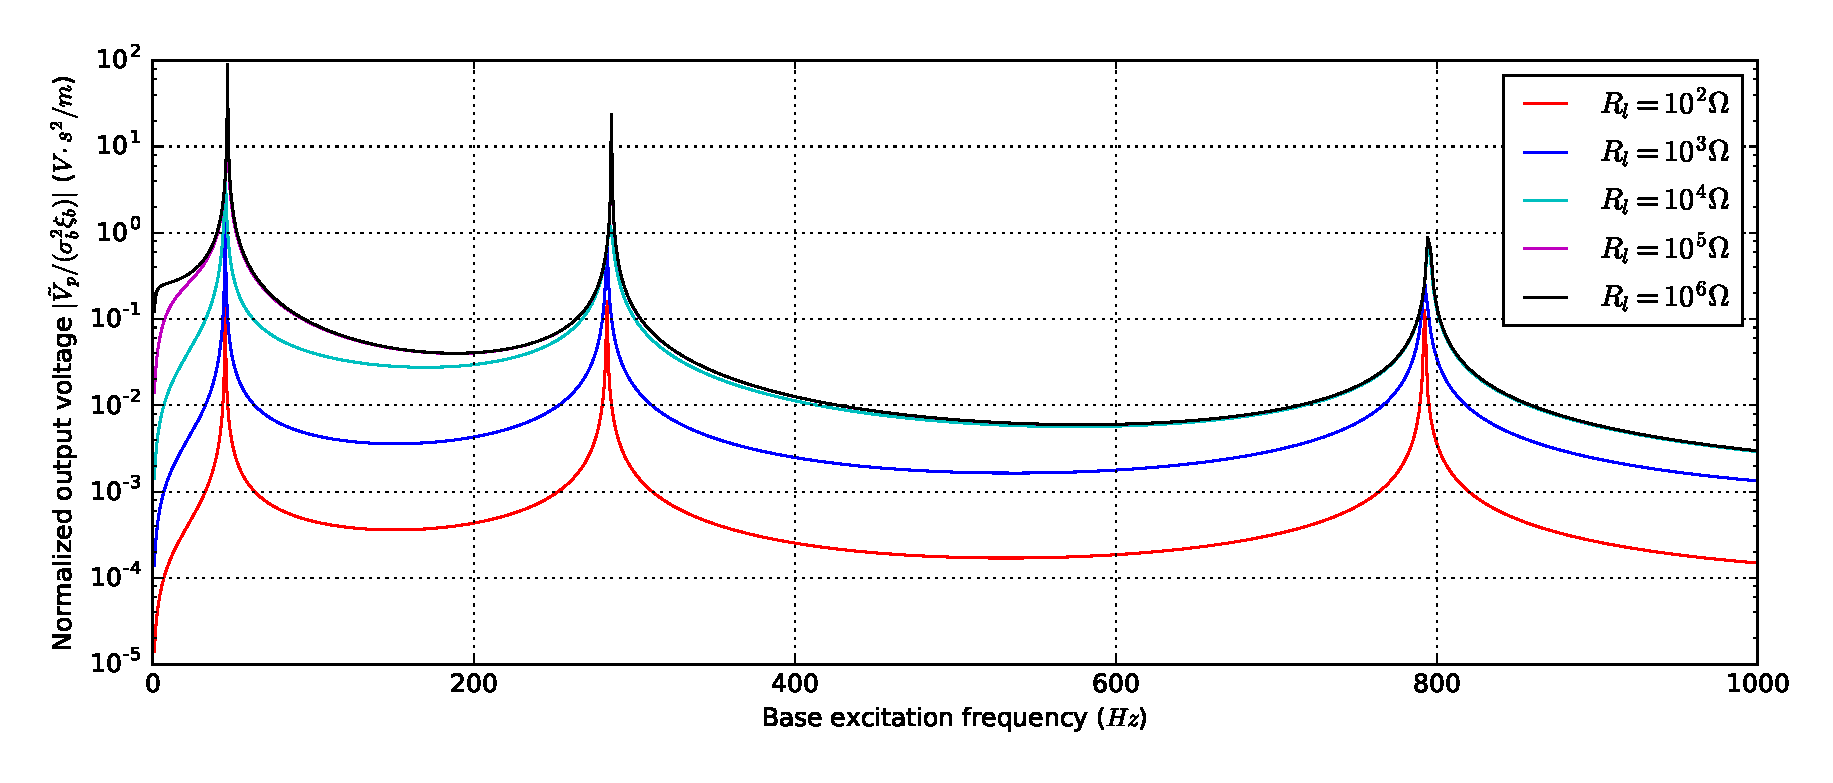
\includegraphics[width=\textwidth]{./img_eig_asy/fig_sol_analytic_perf_vs_fr}
    \caption{Validation calculation of the normalized output voltage versus base excitation frequency for a unimorph piezoelectric cantilever energy harvester based on the data from \cite{erturk2008distributed}.}
    \label{fig:fig_sol_analytic_perf_vs_fr}
\end{figure}

Secondly, according to equations (\ref{eq:eq_disp_func_general_coeffs}) and (\ref{eq:eq_disp_func_coeffs_exps}), the dimensionless displacement amplitude function $u(z)$ is totally determined by the three dimensionless parameters $\sigma$, $\beta$, and $\delta$ introduced before. Among the dimensionless parameters, $\sigma$ is the dimensionless base excitation frequency, $\beta$ is the dimensionless electrical resonant frequency, and $\delta$ is the dimensionless electromechanical coupling strength for the structure. As $\sigma$ and $\beta$ is determined by the base excitation and externally connected circuit respectively, only the parameter $\delta$ is fully determined by the structure itself. Hence we would like to investigate the influence of parameter $\delta$ upon the solution displacement function $u(z)$. By taking different values of $\delta$ , we calculate the displacement amplitude function $u(z)$ and plot the results in Figure~\ref{fig:fig_sol_analytic_disp_fun}.

\begin{figure}[!htbp]
    \centering
    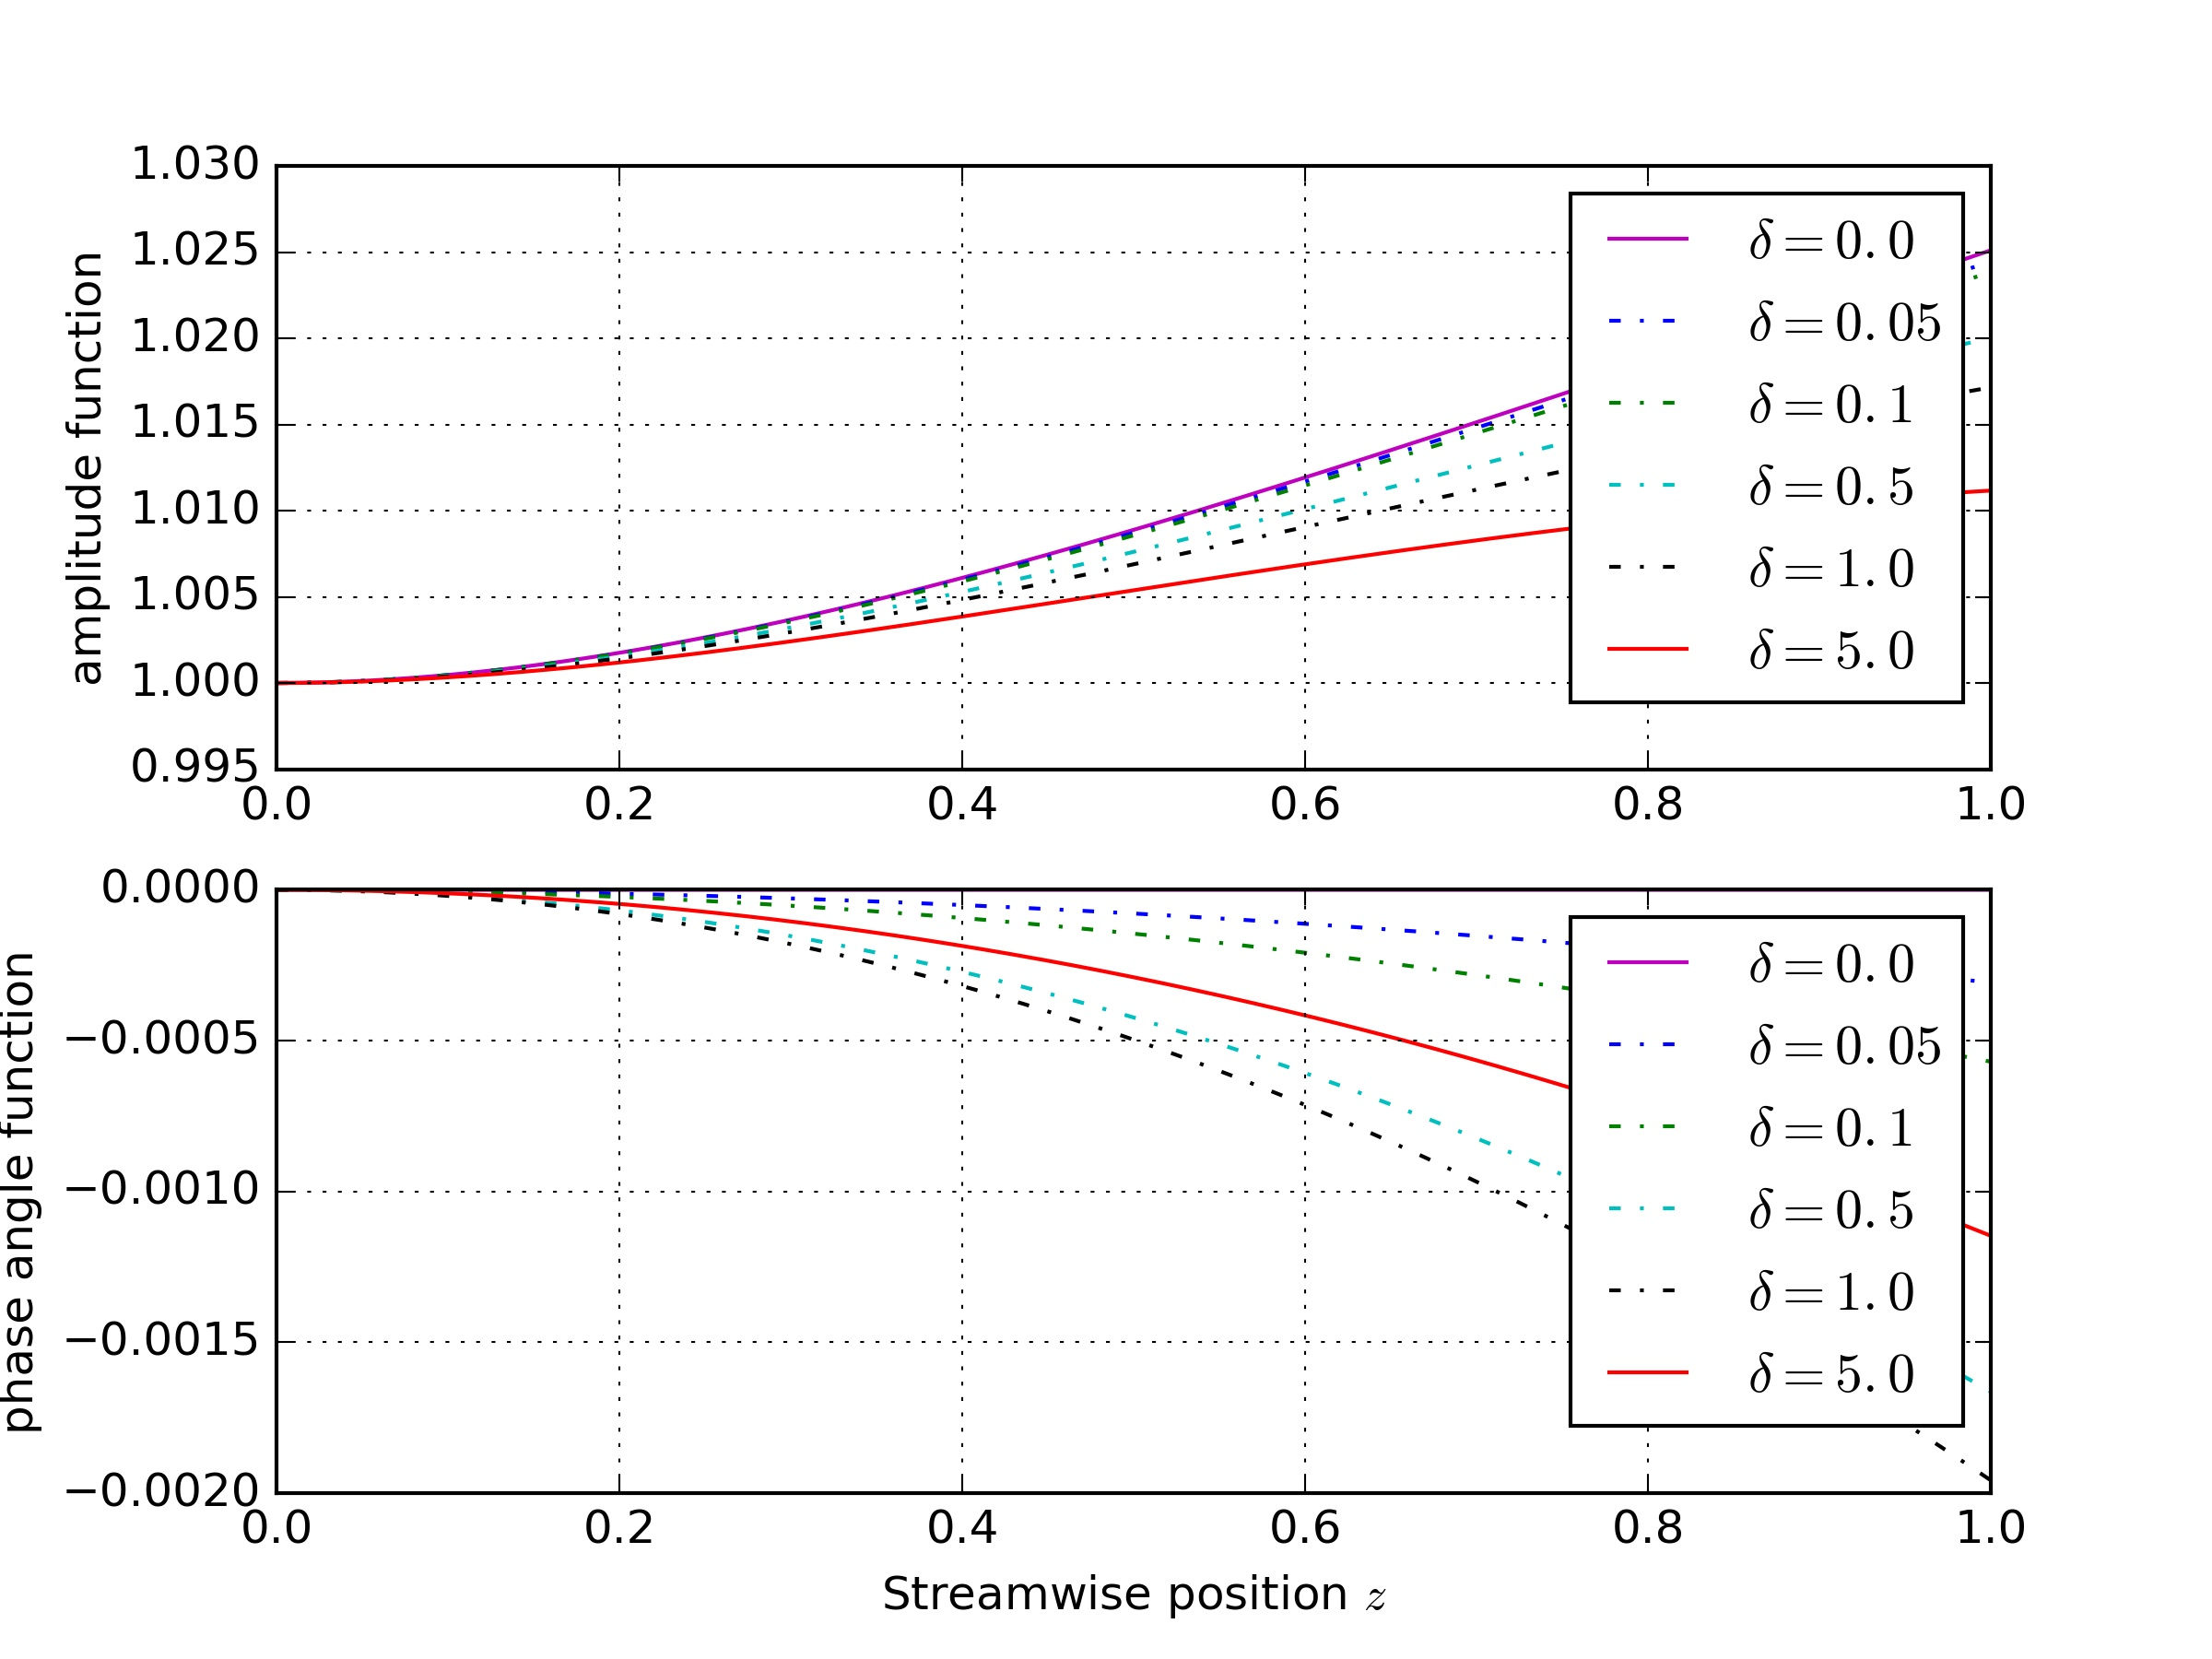
\includegraphics[width=\textwidth]{./img_eig_asy/fig_sol_analytic_disp_fun.jpg}
    \caption{Amplitude and phase of the displacement function $u(z)$ for difference values of $\delta$ }
    \label{fig:fig_sol_analytic_disp_fun}
\end{figure}





It is shown in Figure~\ref{fig:fig_sol_analytic_disp_fun}, the parameter $\delta$ changes the function $u(z)$ through the change of the third boundary condition (\textcolor{red}{to be inserted}). When $\delta$ is zero, i.e., no electromechanical coupling is present, the system degenerates to the classical elastic cantilever beam problem, whose solution is a real function. That is to say, the phase of $u(z)$ is a constant across the whole beam (in the range of $0 \leq z \leq 1$).
Analytical expressions for the coefficients are 
\begin{equation}
    \left\{\begin{aligned}
        A_{\varnothing} &= \frac{ 1 + \cos\sqrt{\sigma } \cosh\sqrt{\sigma } - \sin\sqrt{\sigma } \sinh\sqrt{\sigma} }{2 \left[ 1 + \cos\sqrt{\sigma } \cosh\sqrt{\sigma } \right]}, \\
        B_{\varnothing} &= \frac{ \cos\sqrt{\sigma } \sinh\sqrt{\sigma } + \sin\sqrt{\sigma } \cosh\sqrt{\sigma} }{2 \left[ 1 + \cos\sqrt{\sigma } \cosh\sqrt{\sigma } \right]}, \\
        C_{\varnothing} &= \frac{ 1 + \cos\sqrt{\sigma } \cosh\sqrt{\sigma } + \sin\sqrt{\sigma } \sinh\sqrt{\sigma} }{2 \left[ 1 + \cos\sqrt{\sigma } \cosh\sqrt{\sigma } \right]}, \\
        D_{\varnothing} &= \frac{ -\cos\sqrt{\sigma } \sinh\sqrt{\sigma } - \sin\sqrt{\sigma } \cosh\sqrt{\sigma} }{2 \left[ 1 + \cos\sqrt{\sigma } \cosh\sqrt{\sigma } \right]}.
    \end{aligned}\right.
    \label{eq:eq_disp_func_coeffs_exps_zero}
\end{equation}
and the resulting dimensionless displacement function $u_{\varnothing} (z)$ is represented as
\begin{equation}
    u_{\varnothing} (z) = A_{\varnothing} \cos{\sqrt{\sigma}z} + B_{\varnothing} \sin{\sqrt{\sigma}z} + C_{\varnothing} \cosh{\sqrt{\sigma}z} + D_{\varnothing} \sinh{\sqrt{\sigma}z} - 1.
\end{equation}
When the electromechanical coupling is extremely strong, and $\delta$ is extremely large and can be seen as $\infty$ in mathematical sense. In this situation, the solution $u_\infty (z)$ is again real without any phase difference in the $z$ direction. The coefficients can be analytically expressed as 
\begin{equation}
    \left\{\begin{aligned}
        A_\infty &= \frac{ \cos\sqrt{\sigma } \sinh\sqrt{\sigma } }{ \cos\sqrt{\sigma } \sinh\sqrt{\sigma } + \sin\sqrt{\sigma } \cosh\sqrt{\sigma } }, \\
        B_\infty &= \frac{ \sin\sqrt{\sigma } \sinh\sqrt{\sigma } }{ \cos\sqrt{\sigma } \sinh\sqrt{\sigma } + \sin\sqrt{\sigma } \cosh\sqrt{\sigma } }, \\
        C_\infty &= \frac{ \sin\sqrt{\sigma } \cosh\sqrt{\sigma } }{ \cos\sqrt{\sigma } \sinh\sqrt{\sigma } + \sin\sqrt{\sigma } \cosh\sqrt{\sigma } }, \\
        D_\infty &= \frac{ - \sin\sqrt{\sigma } \sinh\sqrt{\sigma } }{ \cos\sqrt{\sigma } \sinh\sqrt{\sigma } + \sin\sqrt{\sigma } \cosh\sqrt{\sigma } }.
    \end{aligned}\right.
    \label{eq:eq_disp_func_coeffs_exps_infty}
\end{equation}
and hence the dimensionless displacement function $u_{\infty} (z)$ is
\begin{equation}
    u_{\infty} (z) = A_{\infty} \cos{\sqrt{\sigma}z} + B_{\infty} \sin{\sqrt{\sigma}z} + C_{\infty} \cosh{\sqrt{\sigma}z} + D_{\infty} \sinh{\sqrt{\sigma}z} - 1.
\end{equation}
While a finite non-zero electromechanical coupling factor $\delta$ is present, which is expected in most applications, the resulting dimensionless displacement function $u(z)$ has varying magnitude and phase along the stream-wise direction or $z$ direction. Nevertheless, it is seen from the right panel of Figure~\ref{fig:fig_sol_analytic_disp_fun} that for different values of $\delta$, the phase change of $u(z)$ is very small in the $z$ direction, actually in the order $10^{-2}$. 


\begin{figure}[!htbp]
    \centering
    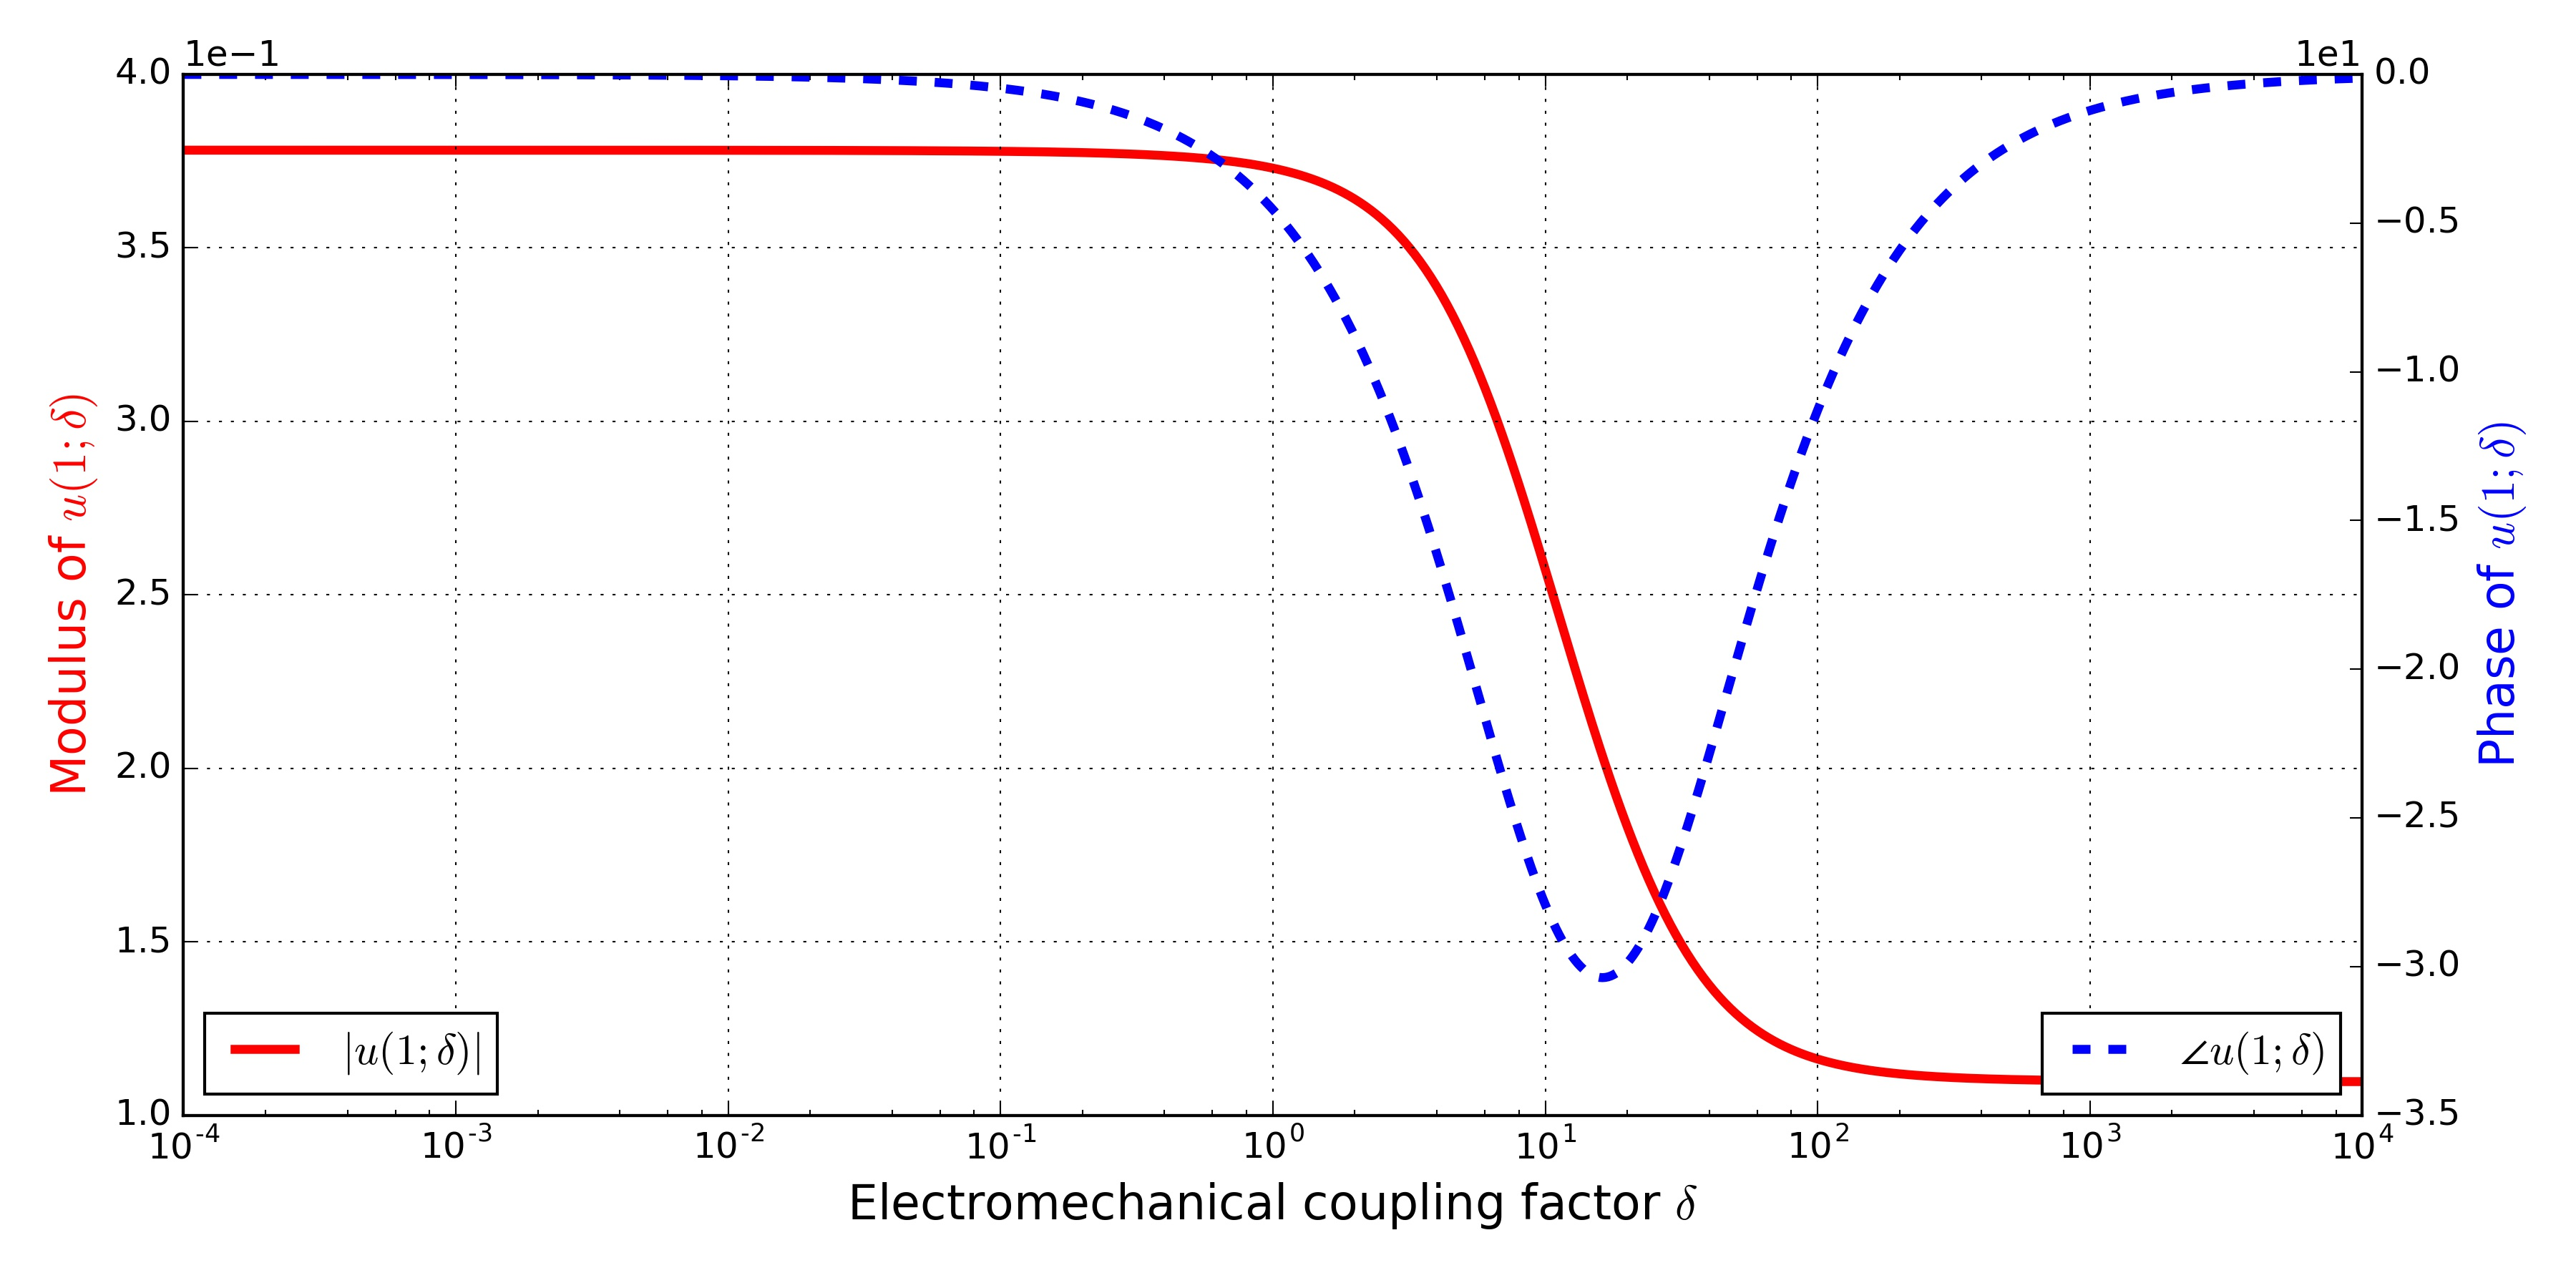
\includegraphics[width=0.8\textwidth]{./img_eig_asy/fig_sol_analytic_disp_end.jpg}
    \caption{Amplitude and phase of the displacement function $u(z)$ at the position $z=1$ versus electromechanical coupling factor $\delta$. }
    \label{fig:fig_sol_analytic_disp_end}
\end{figure}


To make it more clear, we plot the phase of $u(z)$ at $z=1$ versus different values of $\delta$ in Figure~\ref{fig:fig_sol_analytic_disp_end}. It is clear that with the increase of $\delta$, amplitude of the end displamcent $(z=1)$ of the beam $|u(z)|$ decreases, while its phase reaches a minimum at around $\delta = 10$. This also explains the fact expressed in Figure~\ref{fig:fig_sol_analytic_disp_fun} that the amplitude of displacement function $u_\delta (z)$ with $0 < \delta < \infty$ is always between that of $u_\varnothing (z)$ and $u_\infty (z)$.


As for the output voltage $V_p(t)$, output current $I_p(t)$, and output power $P_p(t)$ for the classical piezoelectric cantilever energy harvester, their corresponding complex amplitudes $\tilde{V}_p$, $\tilde{I}_p$, and $\tilde{P}_p$ can be formulated as
\begin{equation}
    \left\{\begin{aligned}
        \tilde{V}_p &= -\frac{j \sigma \beta}{j \sigma \beta + 1} \frac{\eta_b}{l_p} \frac{e_p}{C_p} u^\prime(1), \\
        &= -\frac{j \sigma \beta}{j \sigma \beta + 1} \frac{\eta_b}{l_p} \frac{e_p}{C_p} \sigma^{1/2} \left( - A_\delta \sin{\sqrt{\sigma}} + B_\delta \cos{\sqrt{\sigma}} + C_\delta \sinh{\sqrt{\sigma}} + D_\delta \cosh{\sqrt{\sigma}} \right) \\
        &= - \frac{j \sigma \beta}{j \sigma \beta + 1} \frac{\eta_b}{l_p} \frac{e_p}{C_p}  \frac{ \sqrt{\sigma} \left( \sinh\sqrt{\sigma} - \sin\sqrt{\sigma} \right) }{ 1 + \cos\sqrt{\sigma } \cosh\sqrt{\sigma } + \frac{j \beta \sqrt{\sigma}}{ 1+ j \beta \sigma } \delta \left( \cos\sqrt{\sigma } \sinh\sqrt{\sigma } + \sin\sqrt{\sigma } \cosh\sqrt{\sigma } \right) }\\
        &= - \frac{j \sigma \beta}{j \sigma \beta + 1} \left(\frac{\eta_b}{l_p}\right) \left(\frac{e_p}{C_p}\right) \chi_p , \\
        \tilde{I}_p &=  \tilde{V}_p / R_l = - \frac{ j \sigma \beta } {j \sigma \beta + 1} \left( \frac{\eta_b}{l_p} \right) \left( \frac{e_p}{C_p R_l} \right) \chi_p , \\
        \tilde{P}_p &=  \tilde{V}_p^2 / R_l = \left(\frac{\eta_b}{l_p}\right)^2 \left(\frac{e_p}{C_p}\right) \left( \frac{e_p}{C_p R_l} \right) \left( \frac{ j \sigma \beta}{ j \sigma \beta + 1 } \right)^2 \chi_p^2∫,
    \end{aligned}\right.
    \label{eq:eq_peh_perfs_compact_form}
\end{equation}
in which we have used the notations that 
\begin{equation}
    \chi_p = u_1^\prime(1) = \frac{ \sqrt{\sigma} \left( \sinh\sqrt{\sigma} - \sin\sqrt{\sigma} \right) }{ 1 + \cos\sqrt{\sigma } \cosh\sqrt{\sigma } + \frac{j \beta \sqrt{\sigma}}{ 1+ j \beta \sigma } \delta \left( \cos\sqrt{\sigma } \sinh\sqrt{\sigma } + \sin\sqrt{\sigma } \cosh\sqrt{\sigma } \right) }.
    \label{eq:eq_peh_perfs_compact_form_end_ders}
\end{equation}
Clearly, The three output measures $\tilde{V}_p$, $\tilde{I}_p$, and $\tilde{P}_p$ are heavily dependent on another dimensionless parameter $r_d = \eta_b/l_p$. Formally, both $\tilde{V}_p$ and $\tilde{I}_p$ depend lineary upon $r_d$, while $\tilde{P}_p$ shows a quadratic dependence on $r_d$. The only dependence upon $\delta$ is introduced in $\chi_p$. However, it should be noted that the parameter $\delta$ relies on $e_p$, $l_p$, $C_p$, and $B_p$, while the three measures $\tilde{V}_p$, $\tilde{I}_p$, and $\tilde{P}_p$ are dimensional values and depend on $e_p$, $\sigma_b$, and $R_l$. As a result, the change of parameter $\delta$ results in the change of reference voltage $e_p / C_p$, reference current $e_p / (C_p R_l)$, and reference power $(e_p / C_p)[e_p / (C_p R_l)]$, and therefore the corresponding values of $\tilde{V}_p$, $\tilde{I}_p$, and $\tilde{P}_p$. Hence, we may establish a bijective relation between $\delta$ and $e_p$, and relate the change of $\delta$ to that of $e_p$. In this way, we calculate the output measures at different values of $\delta$ and plot their amplitudes in Figure~\ref{fig:fig_sol_analytic_perf_fun}. 
\begin{figure}[!htbp]
    \centering
    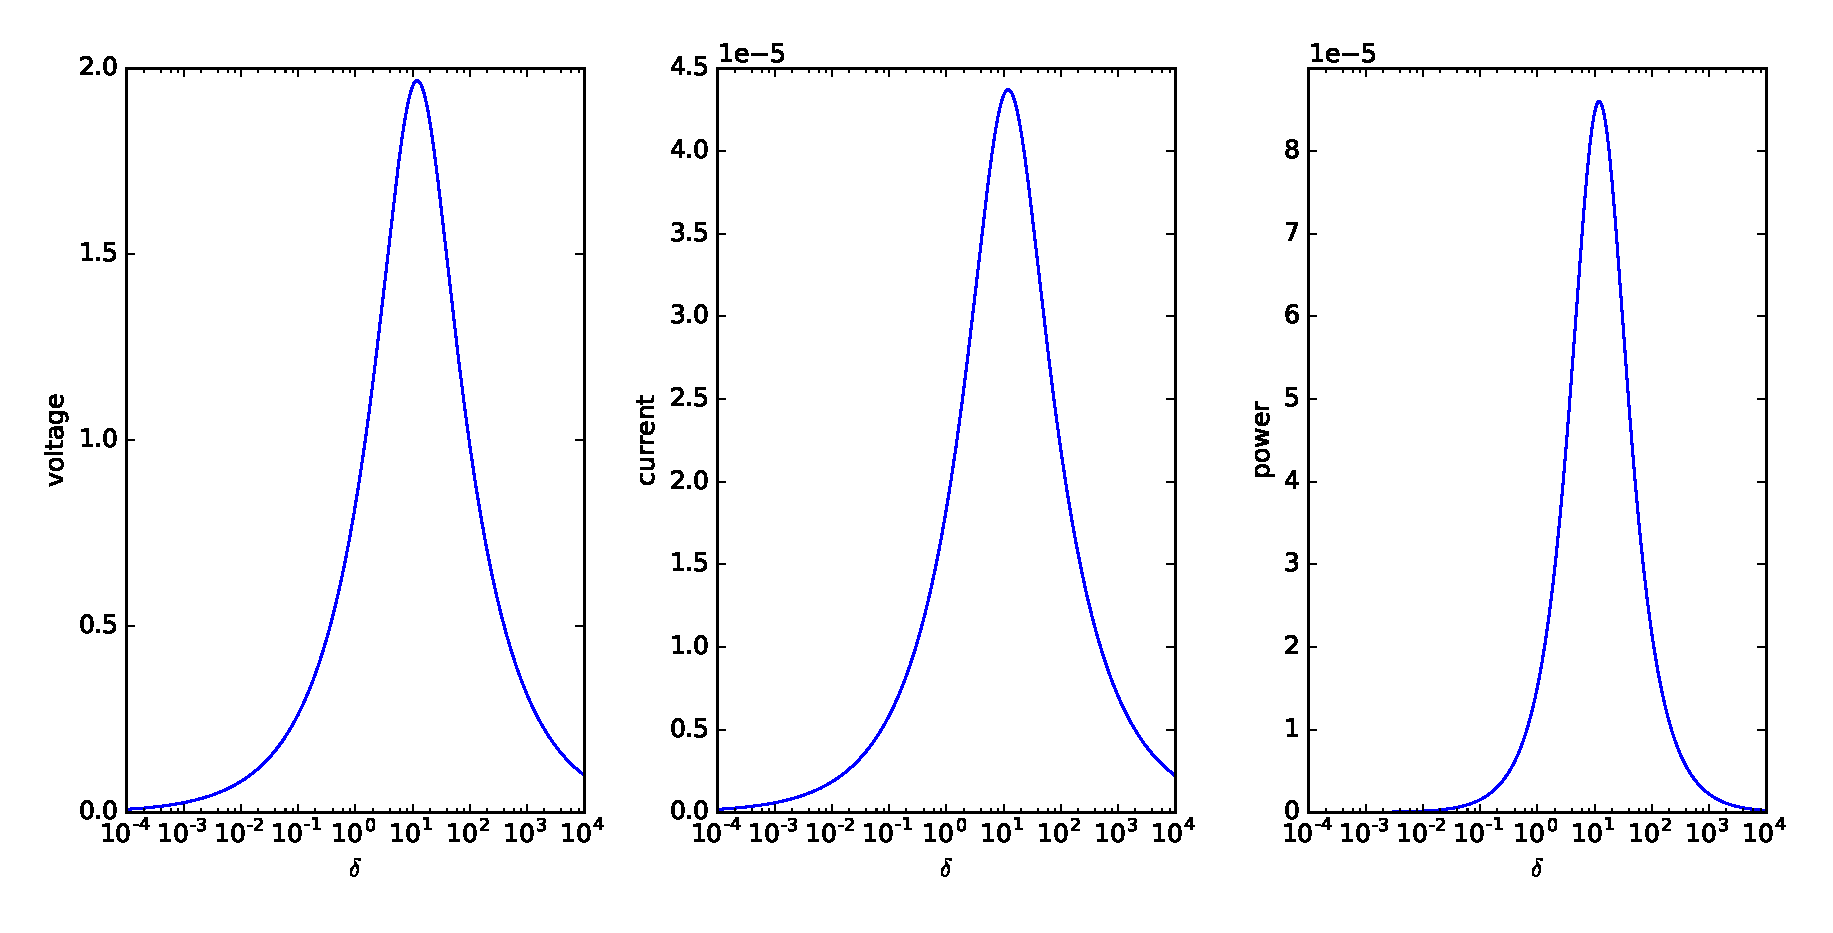
\includegraphics[width=\textwidth]{./img_eig_asy/fig_sol_analytic_perf_fun}
    \caption{Voltage, current and power output for the piezoelectric cantilever energy harvester}
    \label{fig:fig_sol_analytic_perf_fun}
\end{figure}
% For a typical piezoelectric cantilever energy harvester in the literature \cite{erturk2008distributed,erturk2009experimentally}, this parameter $\delta$ is rather small


It is seen from Figure~\ref{fig:fig_sol_analytic_perf_fun} that all the three measures show a maximum peak with the increase of $\delta$ at the approximate value of $\delta = 10$. When $\delta$ is small, or equivalently, $e_p$ is small, amplitude of the three output measures $\tilde{V}_p$, $\tilde{I}_p$, and $\tilde{P}_p$ increase with the increase of $\delta$. Then after the critical value of $\delta$, a further increase of $\delta$ causes the decrease of output measures. Thus we come to a small conclusion that to obtain an optimal output performance, the electromechanical coupling factor $\delta$ should be set to an appropriate value. However, a direct calculation using the parameters introduced in the literature \cite{erturk2008distributed,erturk2009experimentally} shows that the parameter $\delta$ is rather small for a typical piezoelectric cantilever energy harvester. For example, for a piezoelectric voltage constant $e_{31} = -5.35\ C / m^2$, the value of $e_p$ is $-5.35 \times 10^{-5}\ C$, and the final value of $\delta$ is $0.028$. According to the properties of commonly used piezoelectric materials, the parameter $e_{31}$ is always in the range of several or several tens $C / m^2$ \textcolor{red}{reference to be inserted}. That is to say, the final value of $\delta$ can be seen always in the order of $10^{-2}$, which is a rather small value according to the diagram. Hence we could present an asymptotic analysis of the performance of the classical piezoelectric energy harvester. This is the subject of the following section.


\section{Asymptotic analysis of the problem}

Considering that the parameter $\delta$ is small, we expand the theoretical solution to the problem in terms of the small parameter $\delta$ using the following regular expansion:
\begin{equation}
    \left\{\begin{aligned}
        A_\delta &= A_0 + \delta A_1 + \delta^2 A_2 + \cdots, \\
        B_\delta &= B_0 + \delta B_1 + \delta^2 B_2 + \cdots, \\
        C_\delta &= C_0 + \delta C_1 + \delta^2 C_2 + \cdots, \\
        D_\delta &= D_0 + \delta D_1 + \delta^2 D_2 + \cdots. 
    \end{aligned}\right.
\end{equation}
As a result, we obtain the following successive expansion problem:

\noindent
$O(\delta^0)$:
\begin{equation}
    \left\{\begin{aligned}
        A_0 + C_0 &= 1, \\
        B_0 + D_0 &= 0, \\
        - A_0 \cos{\sqrt{\sigma}} - B_0 \sin{\sqrt{\sigma}} + C_0 \cosh{\sqrt{\sigma}} + D_0 \sinh{\sqrt{\sigma}} &= 0, \\
        A_0 \sin{\sqrt{\sigma}} - B_0 \cos{\sqrt{\sigma}} + C_0 \sinh{\sqrt{\sigma}} + D_0 \cosh{\sqrt{\sigma}} &= 0.
    \end{aligned}\right.
\end{equation}
The solution is
\begin{equation}
    \left\{\begin{aligned}
        A_0 &= \frac{1 + \cos\sqrt{\sigma} \cosh\sqrt{\sigma} - \sin\sqrt{\sigma} \sinh\sqrt{\sigma} }{2 + 2 \cos\sqrt{\sigma} \cosh\sqrt{\sigma} }, \\
        B_0 &= \frac{\cosh\sqrt{\sigma} \sin\sqrt{\sigma} + \cos\sqrt{\sigma} \sinh\sqrt{\sigma} }{2 + 2 \cos\sqrt{\sigma} \cosh\sqrt{\sigma} }, \\
        C_0 &= \frac{1 + \cos\sqrt{\sigma} \cosh\sqrt{\sigma} + \sin\sqrt{\sigma} \sinh\sqrt{\sigma} }{2 + 2 \cos\sqrt{\sigma} \cosh\sqrt{\sigma} }, \\
        D_0 &= -\frac{\cosh\sqrt{\sigma} \sin\sqrt{\sigma} + \cos\sqrt{\sigma} \sinh\sqrt{\sigma} }{2 + 2 \cos\sqrt{\sigma} \cosh\sqrt{\sigma} }.
    \end{aligned}\right.
\end{equation}
Hence we have
\begin{equation}
    - A_0 \sin{\sqrt{\sigma}} + B_0 \cos{\sqrt{\sigma}} + C_0 \sinh{\sqrt{\sigma}} + D_0 \cosh{\sqrt{\sigma}} = \frac{\sinh\sqrt{\sigma }-\sin\sqrt{\sigma }}{\cos\sqrt{\sigma } \cosh\sqrt{\sigma }+1}
\end{equation}

\noindent
$O(\delta^1)$:
\begin{equation}
    \left\{\begin{aligned}
        A_1 + C_1 &= 0, \\
        B_1 + D_1 &= 0, \\
        \left( - A_1 \cos{\sqrt{\sigma}} - B_1 \sin{\sqrt{\sigma}} + C_1 \cosh{\sqrt{\sigma}} + D_1 \sinh{\sqrt{\sigma}} \right) &+ \\
        \frac{j \beta \sqrt{\sigma}}{ j\sigma \beta + 1 } \left( - A_0 \sin{\sqrt{\sigma}} + B_0 \cos{\sqrt{\sigma}} + C_0 \sinh{\sqrt{\sigma}} + D_0 \cosh{\sqrt{\sigma}} \right) &= 0, \\
        A_1 \sin{\sqrt{\sigma}} - B_1 \cos{\sqrt{\sigma}} + C_1 \sinh{\sqrt{\sigma}} + D_1 \cosh{\sqrt{\sigma}} &= 0.
    \end{aligned}\right.
\end{equation}
The solution is
\begin{equation}
    \left\{\begin{aligned}
        A_1 &= \frac{j \beta  \sqrt{\sigma }}{1+j \beta  \sigma } \left( \frac{\sinh\sqrt{\sigma }-\sin\sqrt{\sigma }}{\cos\sqrt{\sigma } \cosh\sqrt{\sigma }+1} \right) \left(\frac{\cos\sqrt{\sigma }+\cosh\sqrt{\sigma }}{2 \cos\sqrt{\sigma }\cosh\sqrt{\sigma }+2} \right) \\
        B_1 &= \frac{j \beta  \sqrt{\sigma }}{1+j \beta  \sigma } \left( \frac{\sinh\sqrt{\sigma }-\sin\sqrt{\sigma }}{\cos\sqrt{\sigma } \cosh\sqrt{\sigma }+1} \right) \left( \frac{-\sinh\sqrt{\sigma }+\sin\sqrt{\sigma }}{2 \cos\sqrt{\sigma }\cosh\sqrt{\sigma }+2} \right)\\
        C_1 &= \frac{j \beta  \sqrt{\sigma }}{1+j \beta  \sigma } \left( \frac{\sinh\sqrt{\sigma }-\sin\sqrt{\sigma }}{\cos\sqrt{\sigma } \cosh\sqrt{\sigma }+1} \right) \left( -\frac{\cos\sqrt{\sigma }+\cosh\sqrt{\sigma }}{2 \cos\sqrt{\sigma } \cosh\sqrt{\sigma }+2} \right)\\
        D_1 &= \frac{j \beta  \sqrt{\sigma }}{1+j \beta  \sigma } \left( \frac{\sinh\sqrt{\sigma }-\sin\sqrt{\sigma }}{\cos\sqrt{\sigma } \cosh\sqrt{\sigma }+1} \right) \left( \frac{-\sin\sqrt{\sigma }+\sinh\sqrt{\sigma }}{2 \cos\sqrt{\sigma }\cosh\sqrt{\sigma }+2} \right)
    \end{aligned}\right.
\end{equation}
Then we have
\begin{equation}
    \begin{aligned}
        - A_1 \sin{\sqrt{\sigma}} + B_1 \cos{\sqrt{\sigma}} + C_1 \sinh{\sqrt{\sigma}} + D_1 \cosh{\sqrt{\sigma}} \\
        = \frac{j \beta  \sqrt{\sigma }}{1+j \beta  \sigma } \left(\frac{\sin\sqrt{\sigma } -\sinh\sqrt{\sigma }}{\cos\sqrt{\sigma } \cosh\sqrt{\sigma }+1} \right)  \left( \frac{\cos\sqrt{\sigma } \sinh\sqrt{\sigma }+\sin\sqrt{\sigma } \cosh\sqrt{\sigma }}{\cos\sqrt{\sigma } \cosh\sqrt{\sigma }+1} \right)
    \end{aligned}
\end{equation}

\noindent
$O(\delta^2)$:
\begin{equation}
    \left\{\begin{aligned}
        A_2 + C_2 &= 0, \\
        B_2 + D_2 &= 0, \\
        \left( - A_2 \cos{\sqrt{\sigma}} - B_2 \sin{\sqrt{\sigma}} + C_2 \cosh{\sqrt{\sigma}} + D_2 \sinh{\sqrt{\sigma}} \right) &+ \\
        \frac{j \beta \sqrt{\sigma}}{ j\sigma \beta + 1 } \left( - A_1 \sin{\sqrt{\sigma}} + B_1 \cos{\sqrt{\sigma}} + C_1 \sinh{\sqrt{\sigma}} + D_1 \cosh{\sqrt{\sigma}} \right) &= 0, \\
        A_2 \sin{\sqrt{\sigma}} - B_2 \cos{\sqrt{\sigma}} + C_2 \sinh{\sqrt{\sigma}} + D_2 \cosh{\sqrt{\sigma}} &= 0.
    \end{aligned}\right.
\end{equation}
The solution is
\scriptsize
\begin{equation}
    \left\{\begin{aligned}
        A_2 &= \left( \frac{j \beta \sqrt{\sigma }}{1+j \beta \sigma } \right)^2 \left(\frac{ \sinh\sqrt{\sigma } - \sin\sqrt{\sigma }}{\cos\sqrt{\sigma } \cosh\sqrt{\sigma }+1} \right) \left( \frac{\cos\sqrt{\sigma } \sinh\sqrt{\sigma }+\sin\sqrt{\sigma } \cosh\sqrt{\sigma }}{\cos\sqrt{\sigma } \cosh\sqrt{\sigma }+1} \right) \left(\frac{\cos\sqrt{\sigma }+\cosh\sqrt{\sigma }}{2 \cos\sqrt{\sigma }\cosh\sqrt{\sigma }+2} \right) \\
        B_2 &= \left( \frac{j \beta \sqrt{\sigma }}{1+j \beta \sigma } \right)^2 \left(\frac{\sinh\sqrt{\sigma } - \sin\sqrt{\sigma }}{\cos\sqrt{\sigma } \cosh\sqrt{\sigma }+1} \right) \left( \frac{\cos\sqrt{\sigma } \sinh\sqrt{\sigma }+\sin\sqrt{\sigma } \cosh\sqrt{\sigma }}{\cos\sqrt{\sigma } \cosh\sqrt{\sigma }+1} \right) \left( \frac{-\sinh\sqrt{\sigma }+\sin\sqrt{\sigma }}{2 \cos\sqrt{\sigma }\cosh\sqrt{\sigma }+2} \right)\\
        C_2 &= \left( \frac{j \beta \sqrt{\sigma }}{1+j \beta \sigma } \right)^2 \left(\frac{\sinh\sqrt{\sigma } - \sin\sqrt{\sigma }}{\cos\sqrt{\sigma } \cosh\sqrt{\sigma }+1} \right) \left( \frac{\cos\sqrt{\sigma } \sinh\sqrt{\sigma }+\sin\sqrt{\sigma } \cosh\sqrt{\sigma }}{\cos\sqrt{\sigma } \cosh\sqrt{\sigma }+1} \right) \left( -\frac{\cos\sqrt{\sigma }+\cosh\sqrt{\sigma }}{2 \cos\sqrt{\sigma } \cosh\sqrt{\sigma }+2} \right)\\
        D_2 &= \left( \frac{j \beta \sqrt{\sigma }}{1+j \beta \sigma } \right)^2 \left(\frac{\sinh\sqrt{\sigma } - \sin\sqrt{\sigma }}{\cos\sqrt{\sigma } \cosh\sqrt{\sigma }+1} \right) \left( \frac{\cos\sqrt{\sigma } \sinh\sqrt{\sigma }+\sin\sqrt{\sigma } \cosh\sqrt{\sigma }}{\cos\sqrt{\sigma } \cosh\sqrt{\sigma }+1} \right) \left( \frac{-\sin\sqrt{\sigma }+\sinh\sqrt{\sigma }}{2 \cos\sqrt{\sigma }\cosh\sqrt{\sigma }+2} \right)
    \end{aligned}\right.
\end{equation}
\normalsize

Indeed, we can continue to obtain the coefficients for higher order ($\geq 2$) expansions, as shown in the appendices (\textcolor{red}{To add some comments}) using successive iteration method. Nevertheless, it suffices here to consider up to the second order expansion $u^{(0)} (z)$, $u^{(1)} (z)$, and $u^{(2)} (z)$, respectively:
\begin{equation}
    \left\{\begin{aligned}
        u^{(0)} (z) &= u_0 (z), \\
        u^{(1)} (z) &= u_0 (z) + \delta u_1(z), \\
        u^{(2)} (z) &= u_0 (z) + \delta u_1(z) + \delta^2 u_2 (z),
    \end{aligned}\right.
\end{equation}
where the terms $u_0 (z)$, $u_1(z)$, and $u_2 (z)$ are defined as
\begin{equation}
    \left\{\begin{aligned}
        u_0 (z) &= A_0 \cos{\sqrt{\sigma}z} + B_0 \sin{\sqrt{\sigma}z} + C_0 \cosh{\sqrt{\sigma}z} + D_0 \sinh{\sqrt{\sigma}z} - 1, \\
        u_1 (z) &= A_1 \cos{\sqrt{\sigma}z} + B_1 \sin{\sqrt{\sigma}z} + C_1 \cosh{\sqrt{\sigma}z} + D_1 \sinh{\sqrt{\sigma}z}, \\
        u_2 (z) &= A_2 \cos{\sqrt{\sigma}z} + B_2 \sin{\sqrt{\sigma}z} + C_2 \cosh{\sqrt{\sigma}z} + D_2 \sinh{\sqrt{\sigma}z}.
    \end{aligned}\right.
\end{equation}


For different values of $\delta$ and $\sigma$ (Here in this simulation, the value of $\sigma$ is changed through the variance of base excitation frequency $f_b$), the asymptotic approximations of the dimensionless relative beam displacement function $u(z;\delta)$ up to the second order $u^{(0)}(z)$, $u^{(1)}(z)$, and $u^{(2)}(z)$ are calculated and compared to the closed solution $u(z;\delta)$ itself. The results are shown in Figure~\ref{fig:fig_sol_analytic_disp_cmp_fr001}, \ref{fig:fig_sol_analytic_disp_cmp_fr020}, \ref{fig:fig_sol_analytic_disp_cmp_fr040}, \ref{fig:fig_sol_analytic_disp_cmp_fr045}, \ref{fig:fig_sol_analytic_disp_cmp_fr060}, \ref{fig:fig_sol_analytic_disp_cmp_fr080}, \ref{fig:fig_sol_analytic_disp_cmp_fr100}. 


\begin{figure}[!htbp]
    \centering
    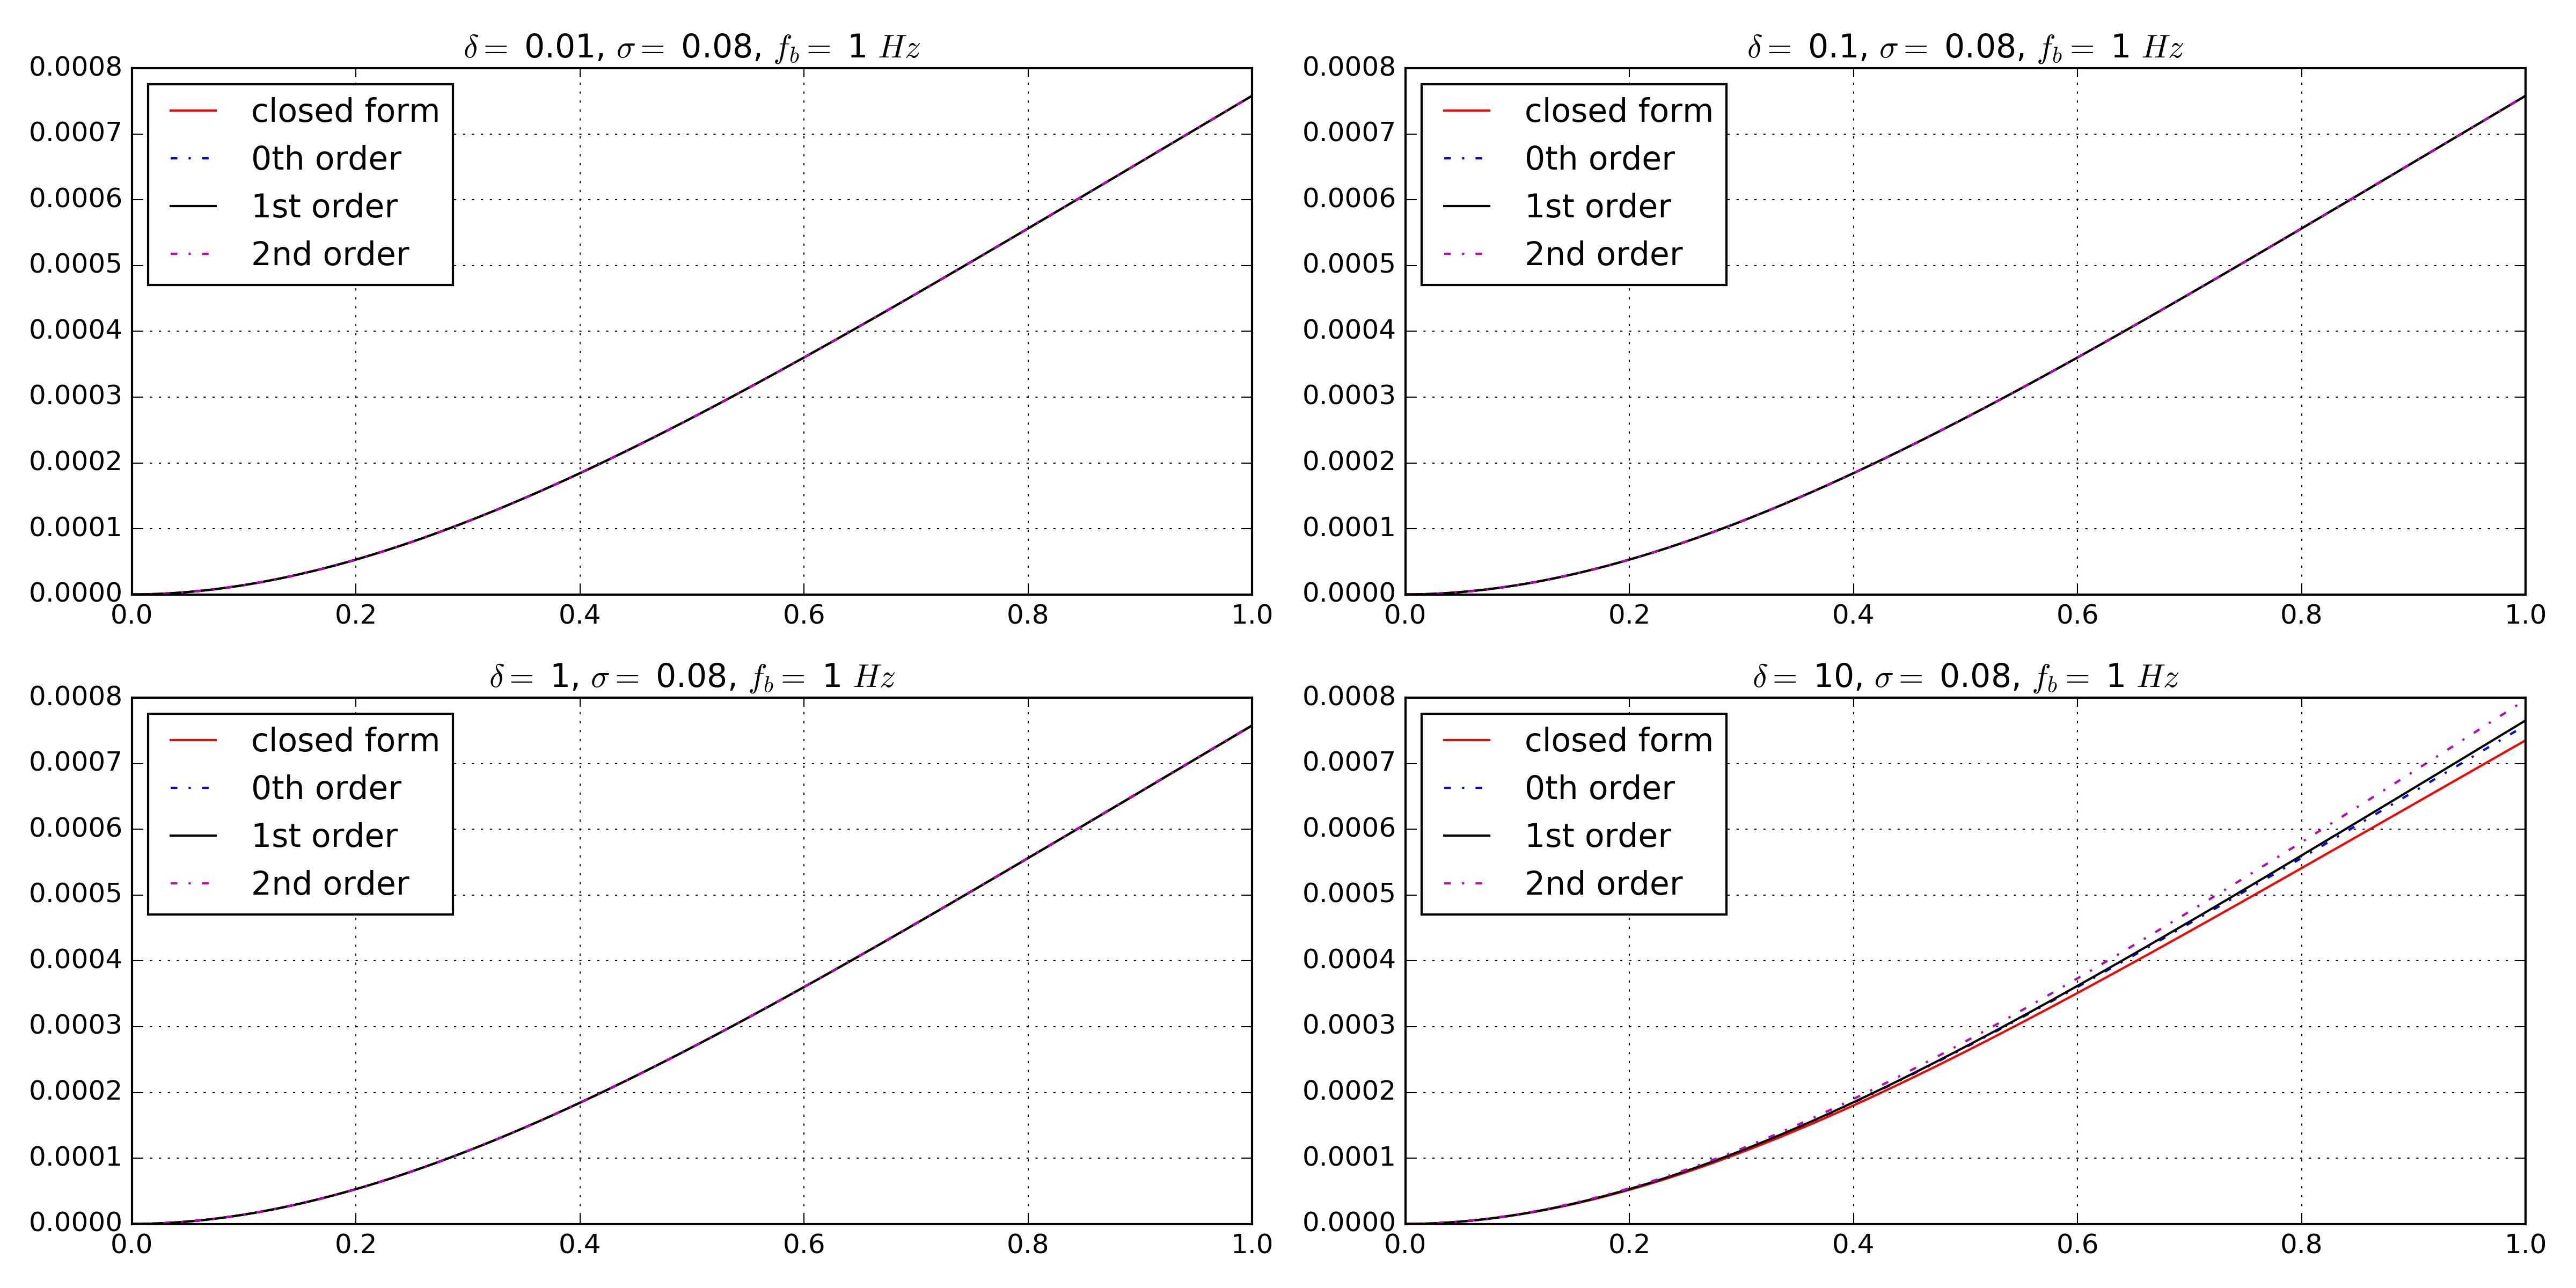
\includegraphics[width=\textwidth]{./img_eig_asy/fig_sol_analytic_disp_cmp_fr001}
    \caption{Comparison for the different orders of asymptotic expansion for the dimensionless relative displacement function $u_\delta(z)$.}
    \label{fig:fig_sol_analytic_disp_cmp_fr001}
\end{figure}



Notice from Figure~\ref{fig:fig_sol_analytic_perf_vs_fr} that the first mode resonant frequency for the device is around $45\ Hz$. It is seen from these results that a smaller value of $\delta$ results in a better approximation, whatever the value of $f_b$. This is consistent with the philosophy behind asymptotic expansion. Besides, for the frequency away from the resonant frequency, the approximation results are relatively accurate in the range of $\delta \leq 0.1$ depending on the value of $f_b$. While when the base exciation frequency $f_b$ is close to a resonance, for exmaple $f_b = 45\ Hz$, the approximation results are not accurate even at the value of $\delta = 0.01$. That is to say, the asymptotic expansion in terms of $\delta$ is not uniform with respect to parameter $\sigma$. Especially, the existence of resonance actually restrict the behavior of the asymptotic expansion. Around the resonance the expansion will show low accuracy, while away from the resonance, the expansion accuracy is easily retained. Nonetheless, for commonly used piezoelectric materials and energy harvesting device configuration, the value of $\delta$ is usually in the range of $10^{-2}$. Hence, it is generally validated to use the asymptotic expansion method to approximate the dimensionless displacement function $u(z;\delta)$. Furtherly, in view of the aprroximating performances of the asymptotic expansions to different orders, it suffices to keep only the $0th$ order terms. Then, we have that 
\begin{equation}
    u(z;\delta) \approx u^{(0)}(z) = A_0 \cos{\sqrt{\sigma}z} + B_0 \sin{\sqrt{\sigma}z} + C_0 \cosh{\sqrt{\sigma}z} + D_0 \sinh{\sqrt{\sigma}z} - 1.
\end{equation}


\begin{figure}[!htbp]
    \centering
    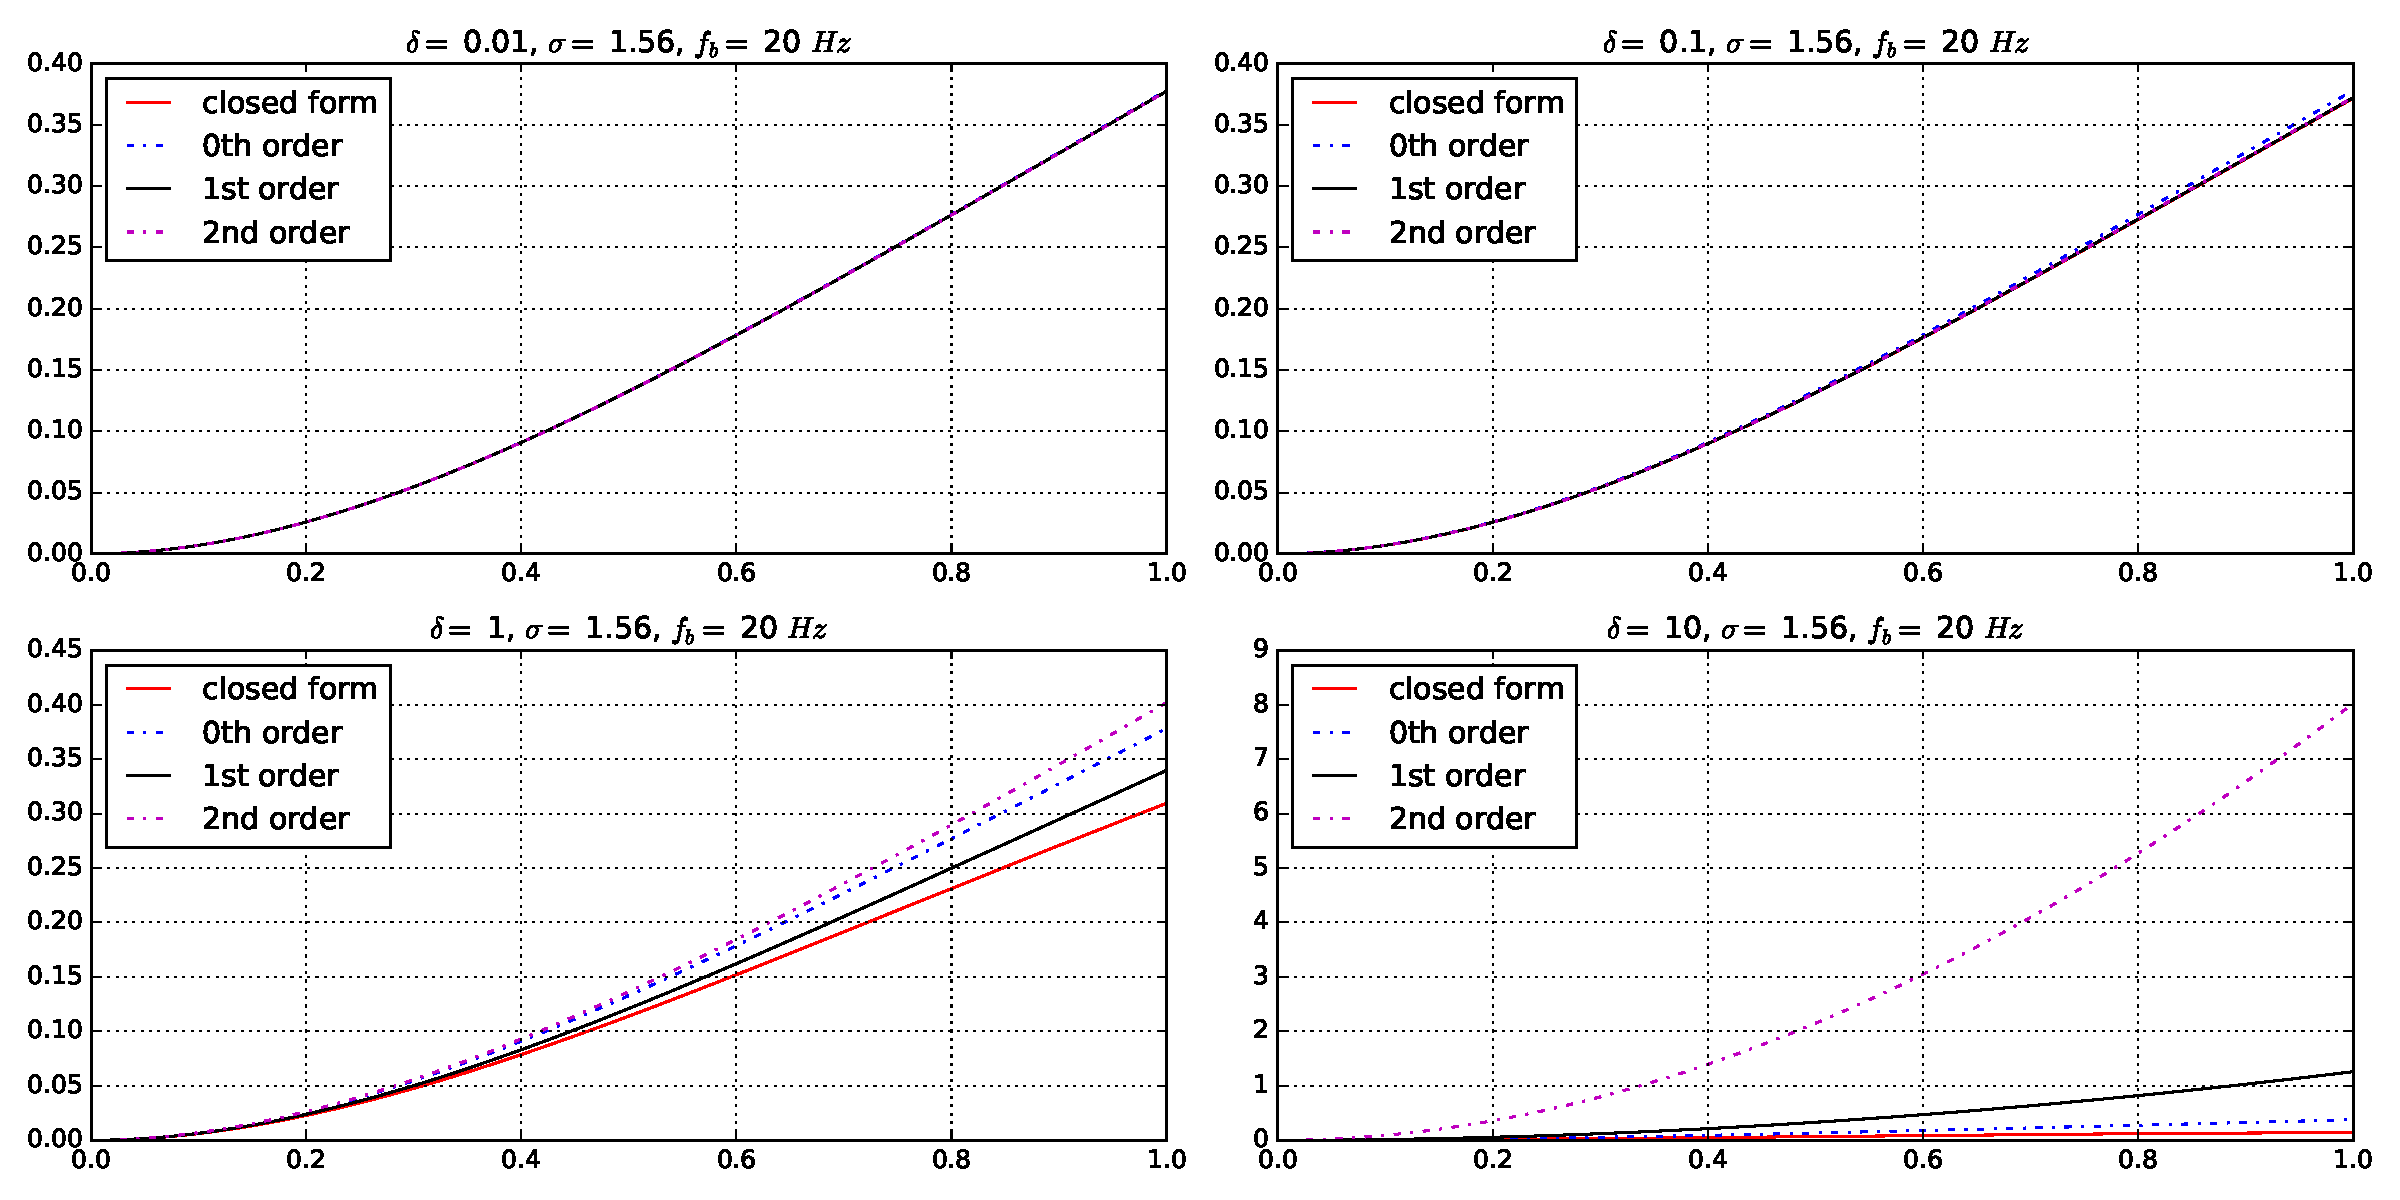
\includegraphics[width=\textwidth]{./img_eig_asy/fig_sol_analytic_disp_cmp_fr020}
    \caption{Comparison for the different orders of asymptotic expansion for the dimensionless relative displacement function $u_\delta(z)$.}
    \label{fig:fig_sol_analytic_disp_cmp_fr020}
\end{figure}


This is exactly the displacement function of a pure elastic cantilever beam. It means that for most piezoelectric energy harvesting devices, due to the fact that the electromechanical coupling factor is relatively small, the displacement function is not much affected. In this way, we have indeed uncoupled the electrical part and elastic part of a piezoelectric energy harvesting device. It should be noted that the approximation is not valid near the resonant points.





\begin{figure}[!htbp]
    \centering
    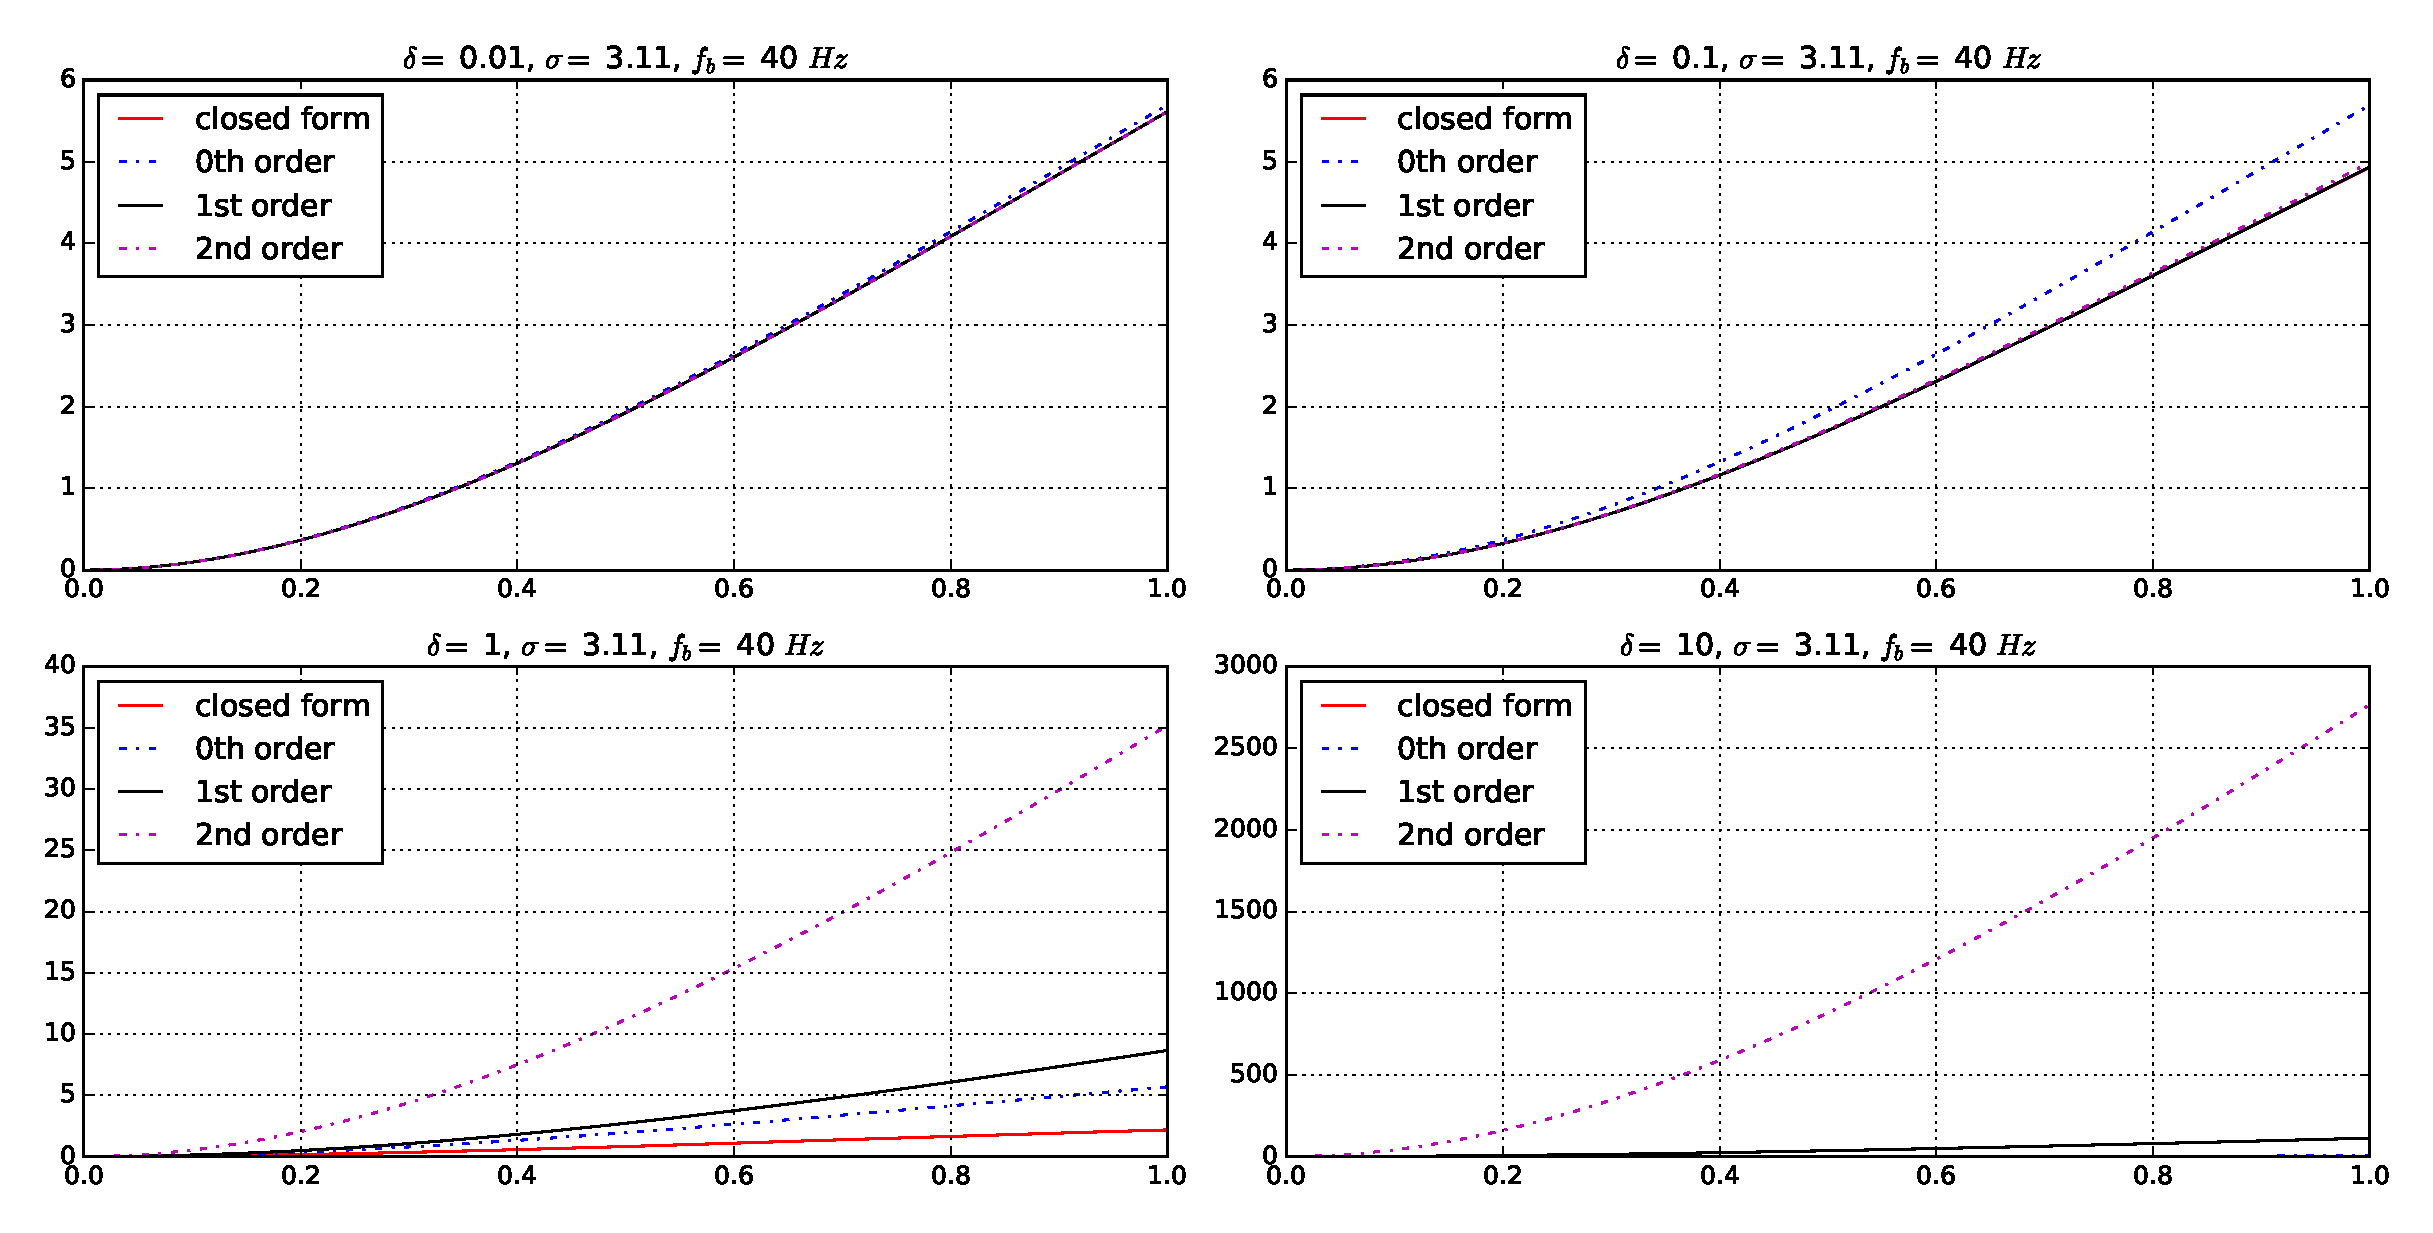
\includegraphics[width=\textwidth]{./img_eig_asy/fig_sol_analytic_disp_cmp_fr040}
    \caption{Comparison for the different orders of asymptotic expansion for the dimensionless relative displacement function $u_\delta(z)$.}
    \label{fig:fig_sol_analytic_disp_cmp_fr040}
\end{figure}


\begin{figure}[!htbp]
    \centering
    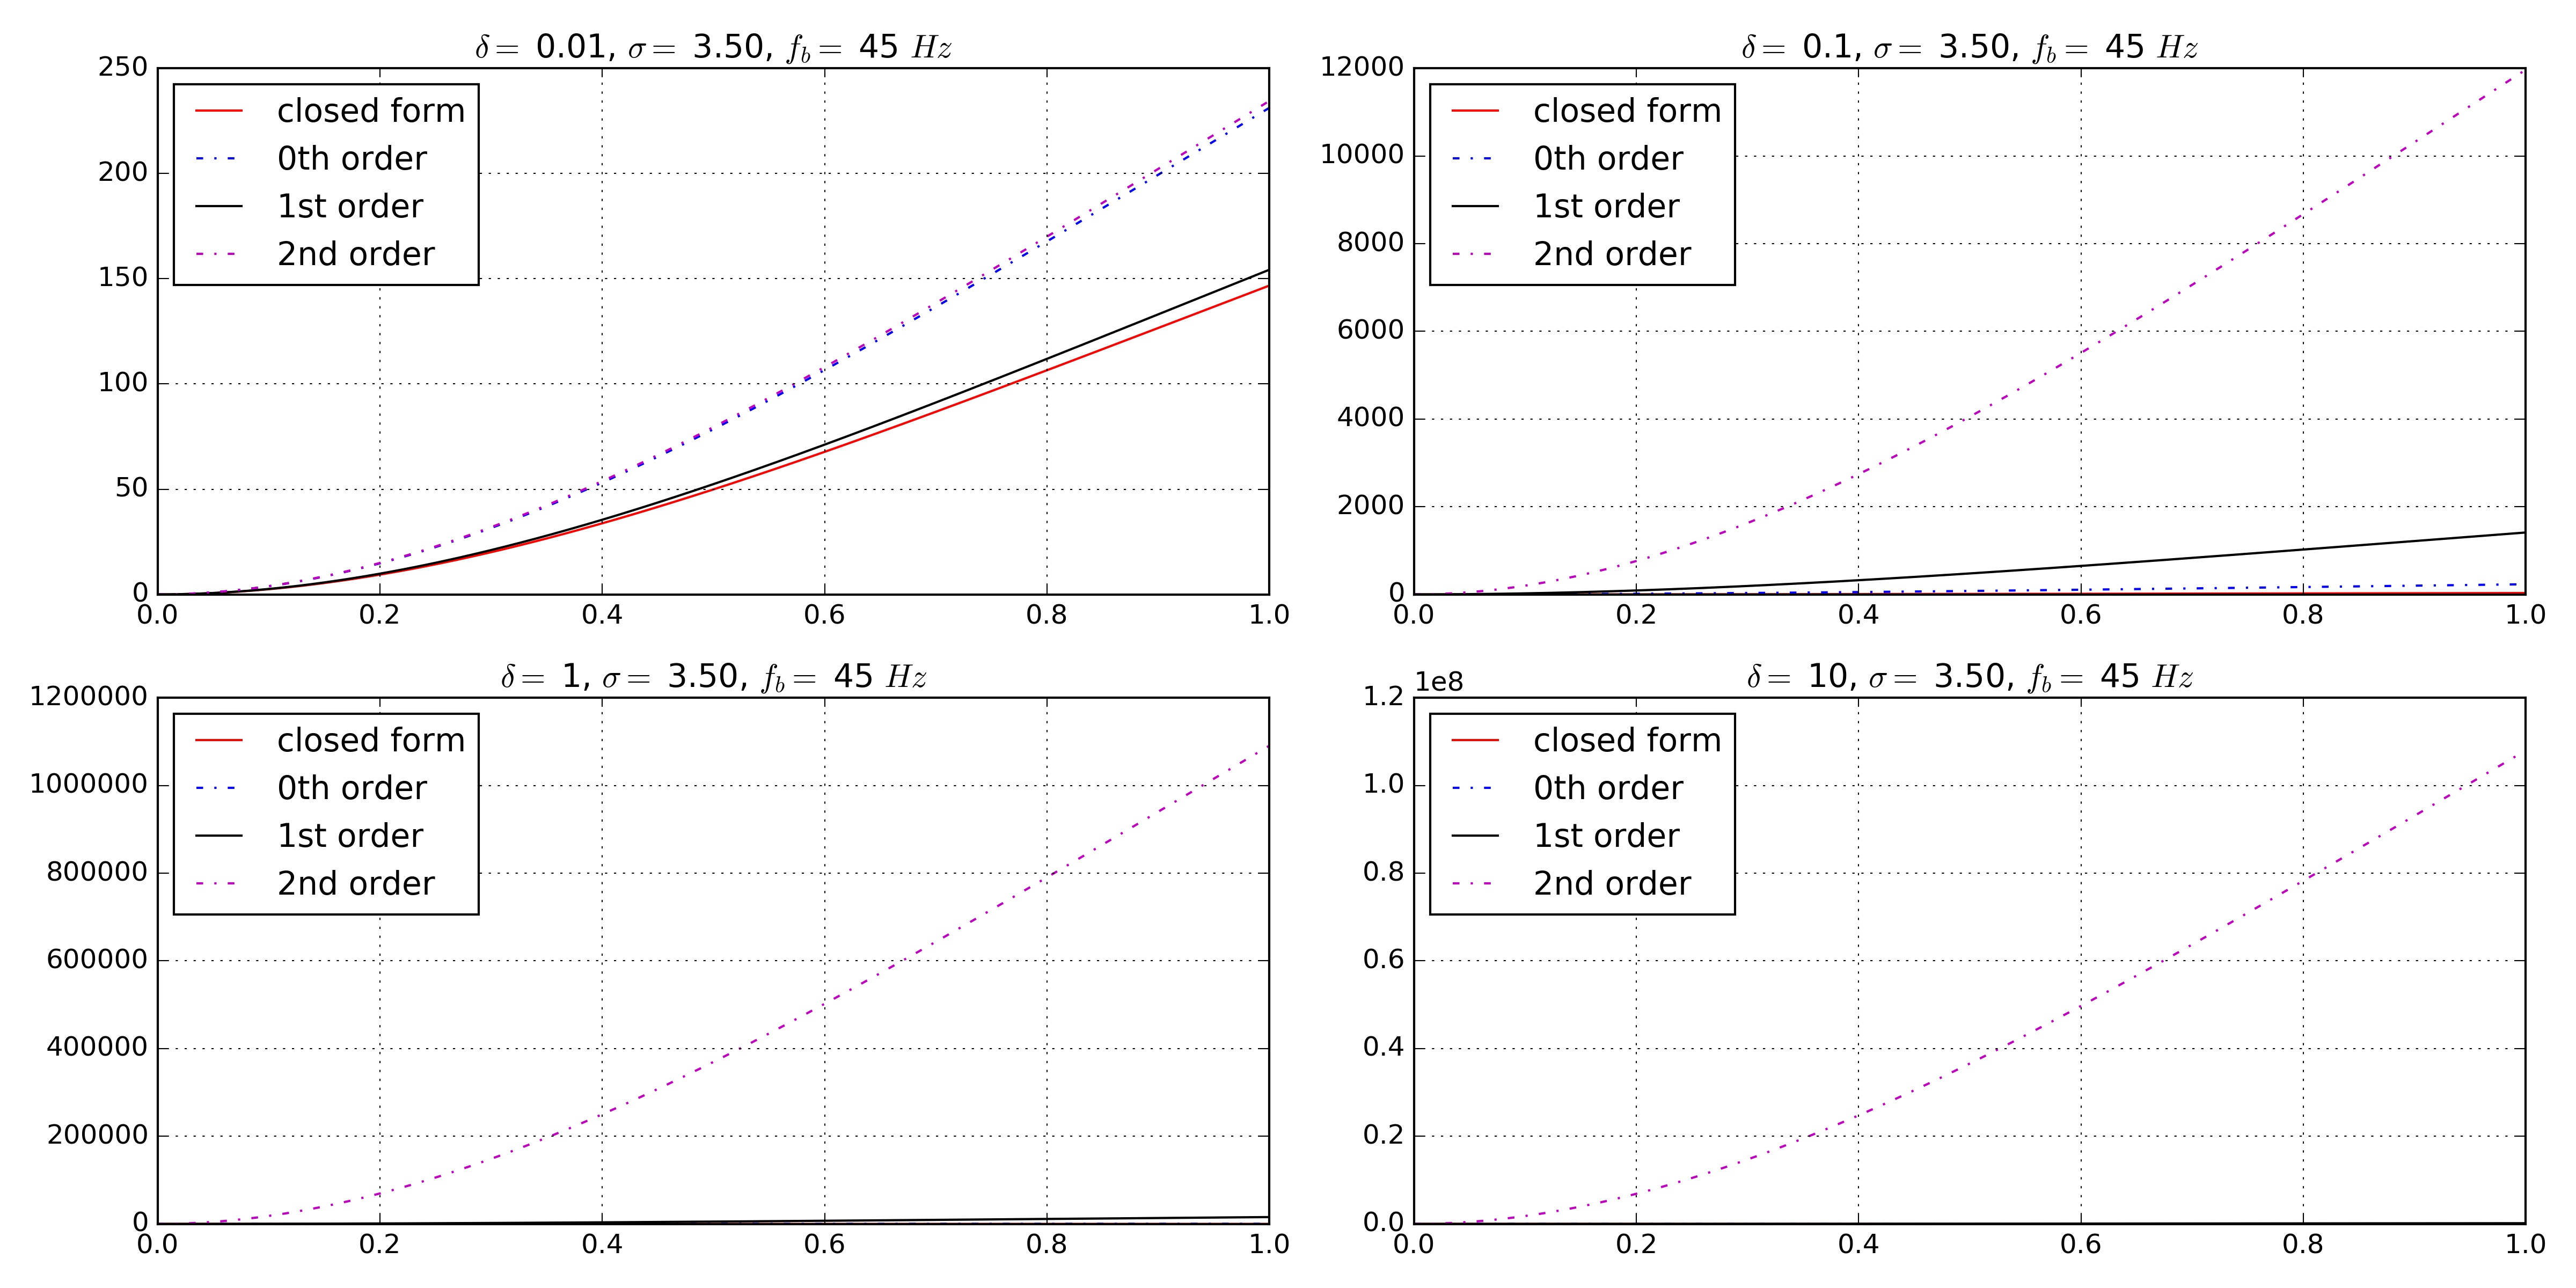
\includegraphics[width=\textwidth]{./img_eig_asy/fig_sol_analytic_disp_cmp_fr045}
    \caption{Comparison for the different orders of asymptotic expansion for the dimensionless relative displacement function $u_\delta(z)$.}
    \label{fig:fig_sol_analytic_disp_cmp_fr045}
\end{figure}


\begin{figure}[!htbp]
    \centering
    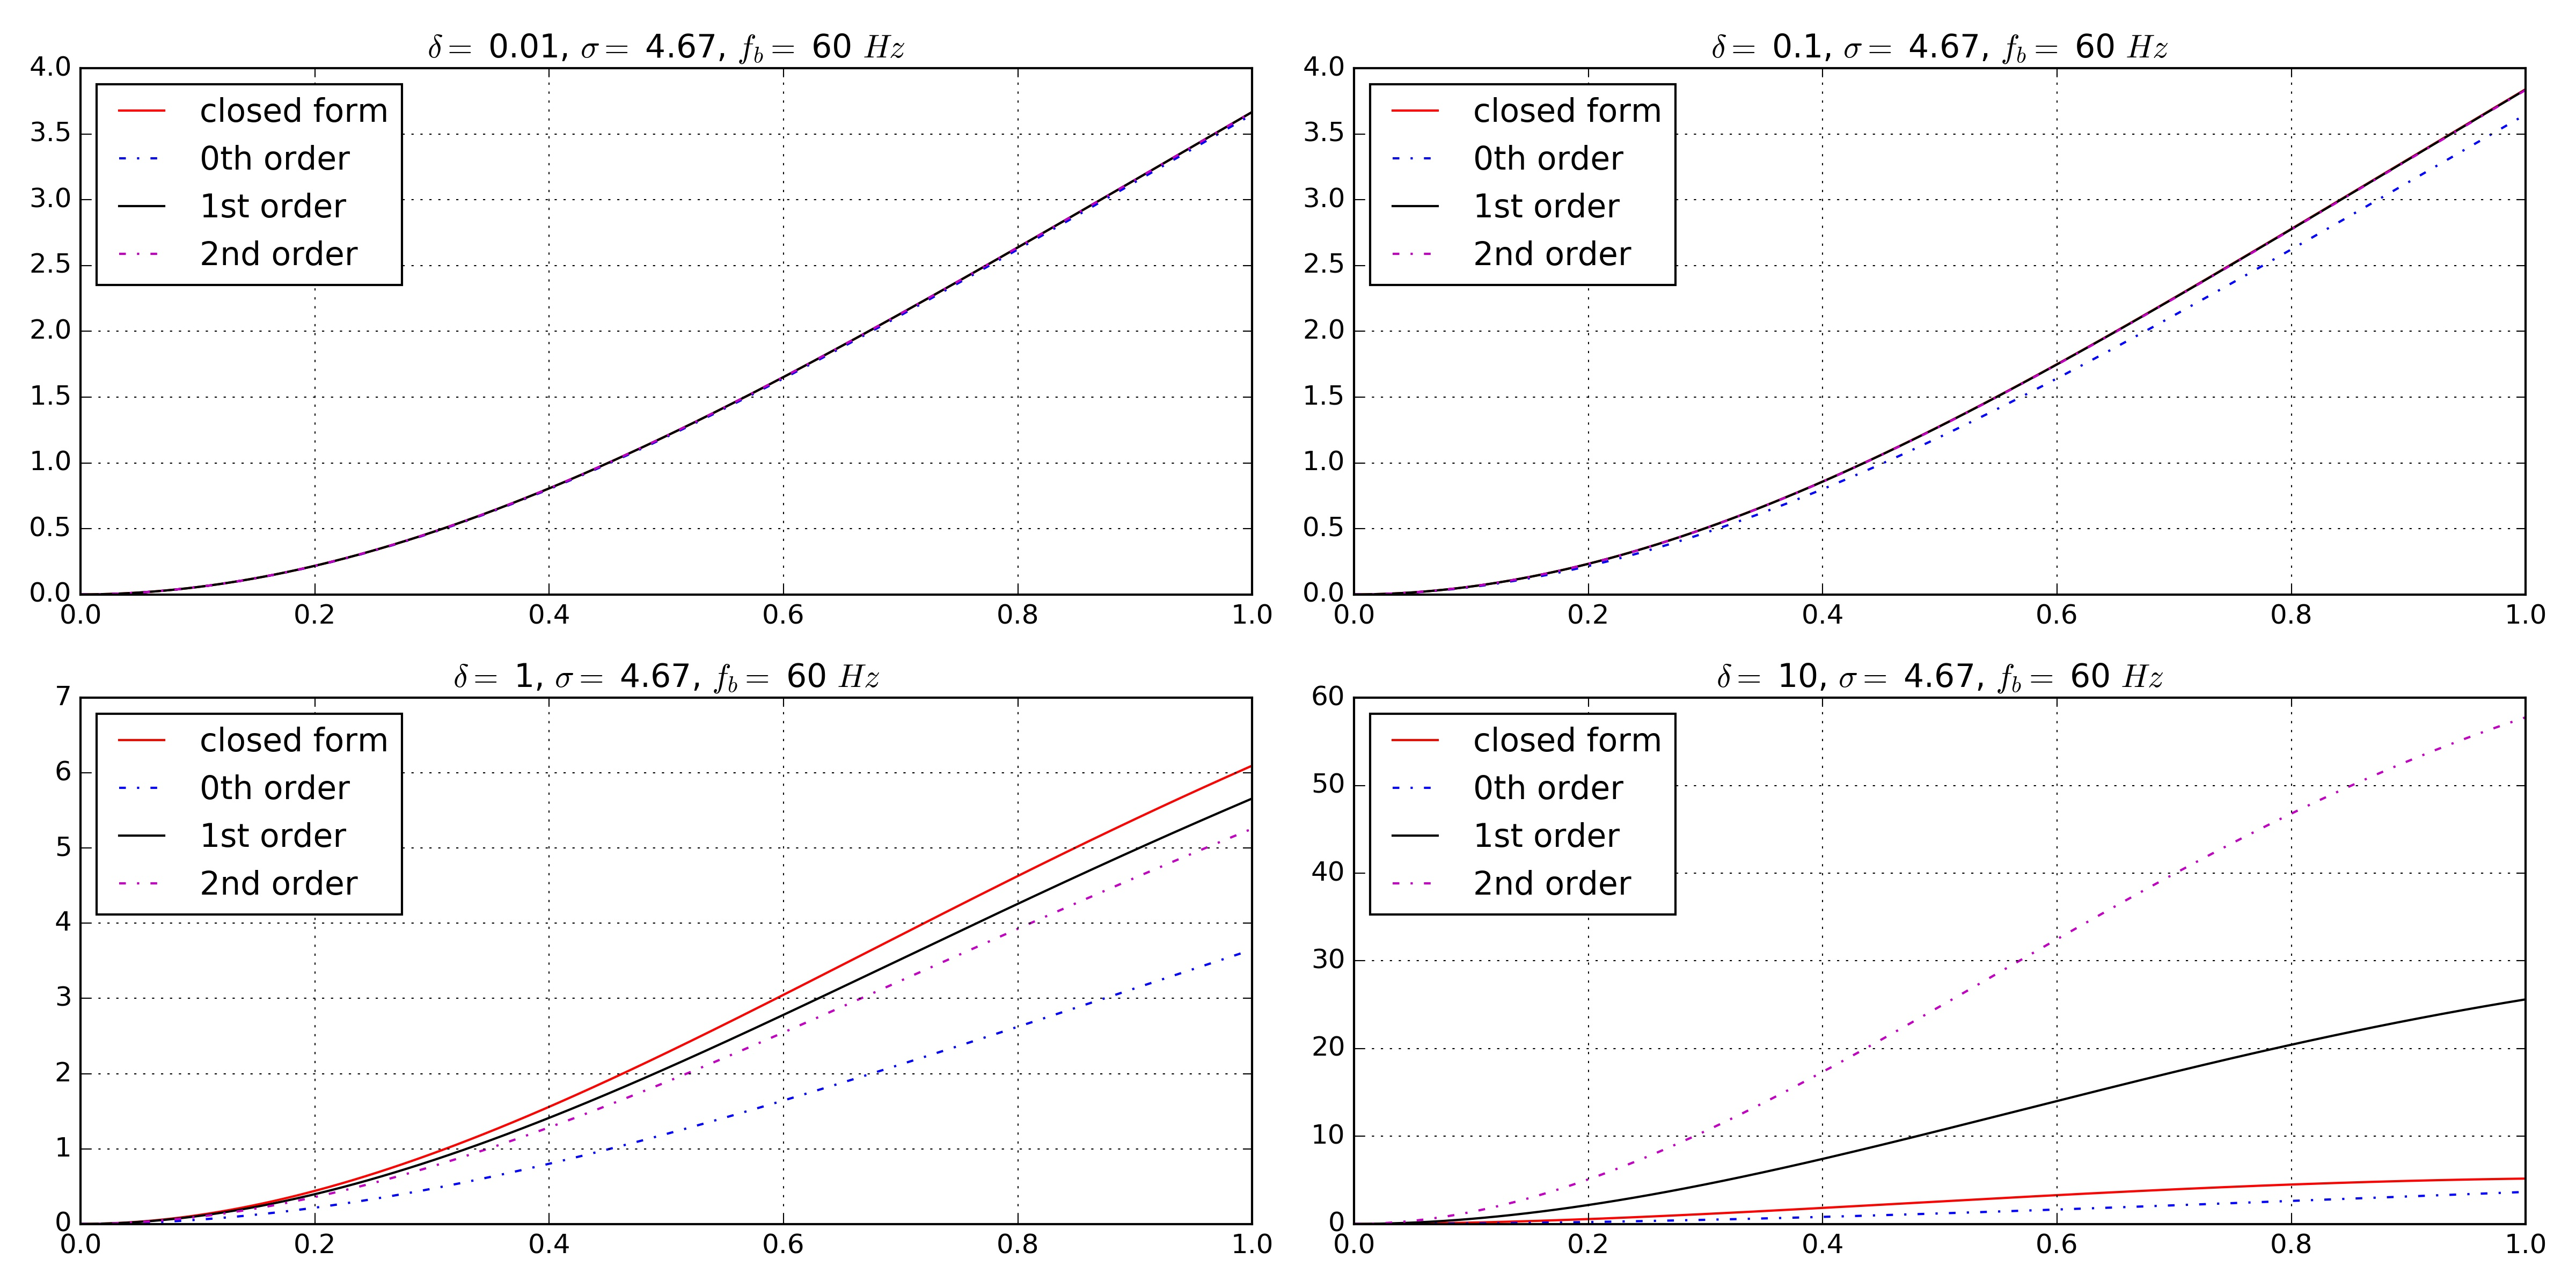
\includegraphics[width=\textwidth]{./img_eig_asy/fig_sol_analytic_disp_cmp_fr060}
    \caption{Comparison for the different orders of asymptotic expansion for the dimensionless relative displacement function $u_\delta(z)$.}
    \label{fig:fig_sol_analytic_disp_cmp_fr060}
\end{figure}


\begin{figure}[!htbp]
    \centering
    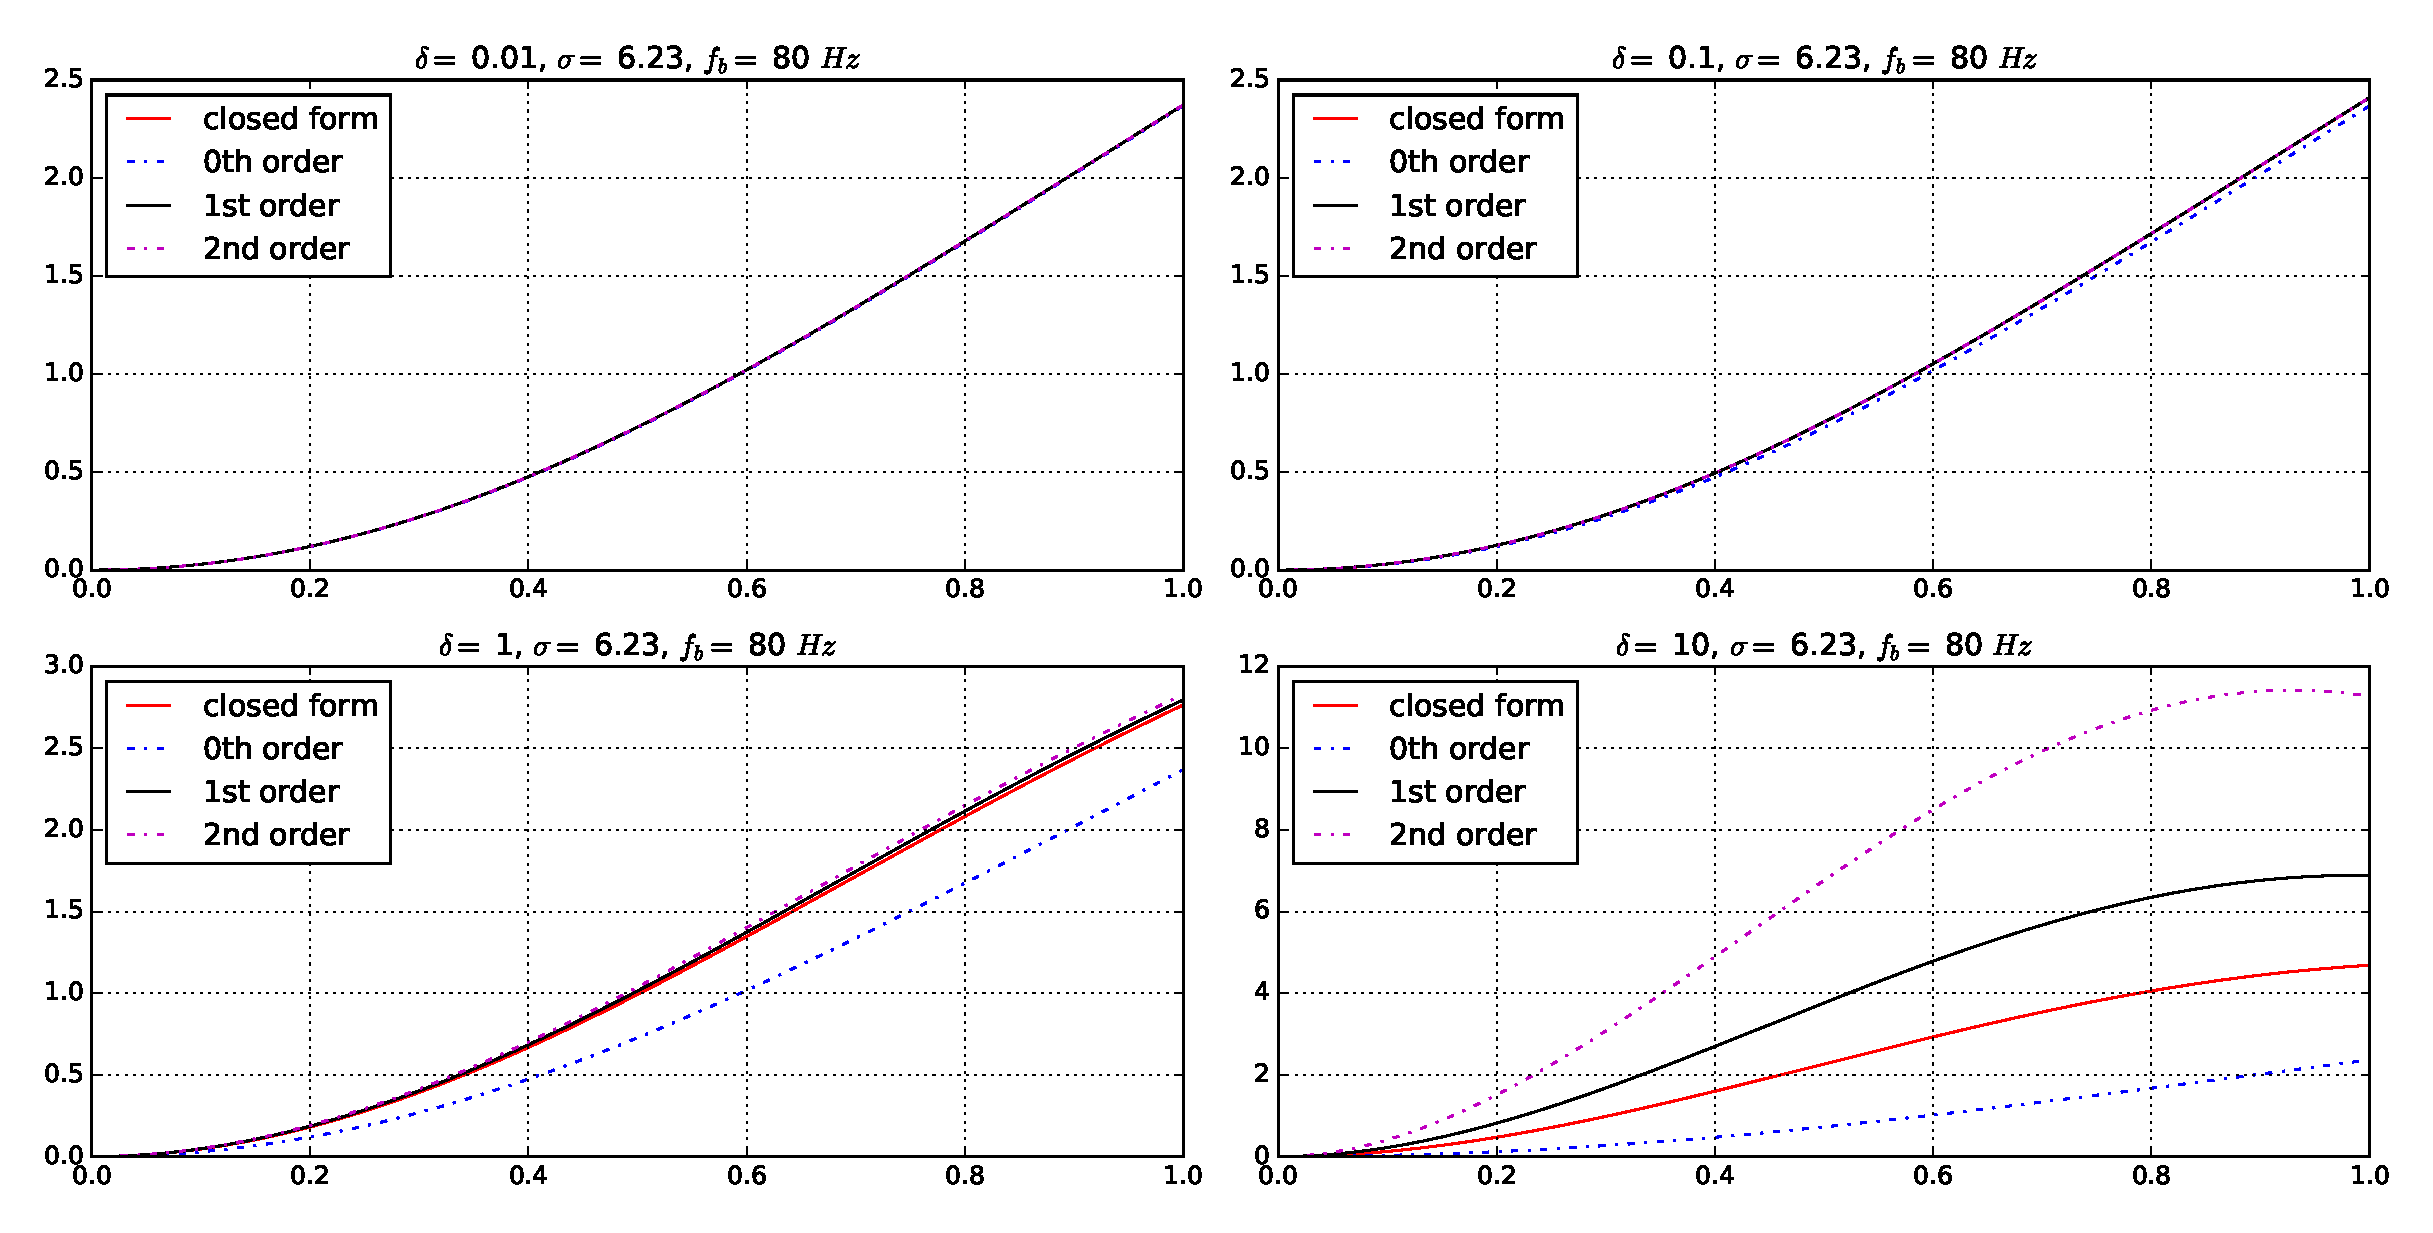
\includegraphics[width=\textwidth]{./img_eig_asy/fig_sol_analytic_disp_cmp_fr080}
    \caption{Comparison for the different orders of asymptotic expansion for the dimensionless relative displacement function $u_\delta(z)$.}
    \label{fig:fig_sol_analytic_disp_cmp_fr080}
\end{figure}


\begin{figure}[!htbp]
    \centering
    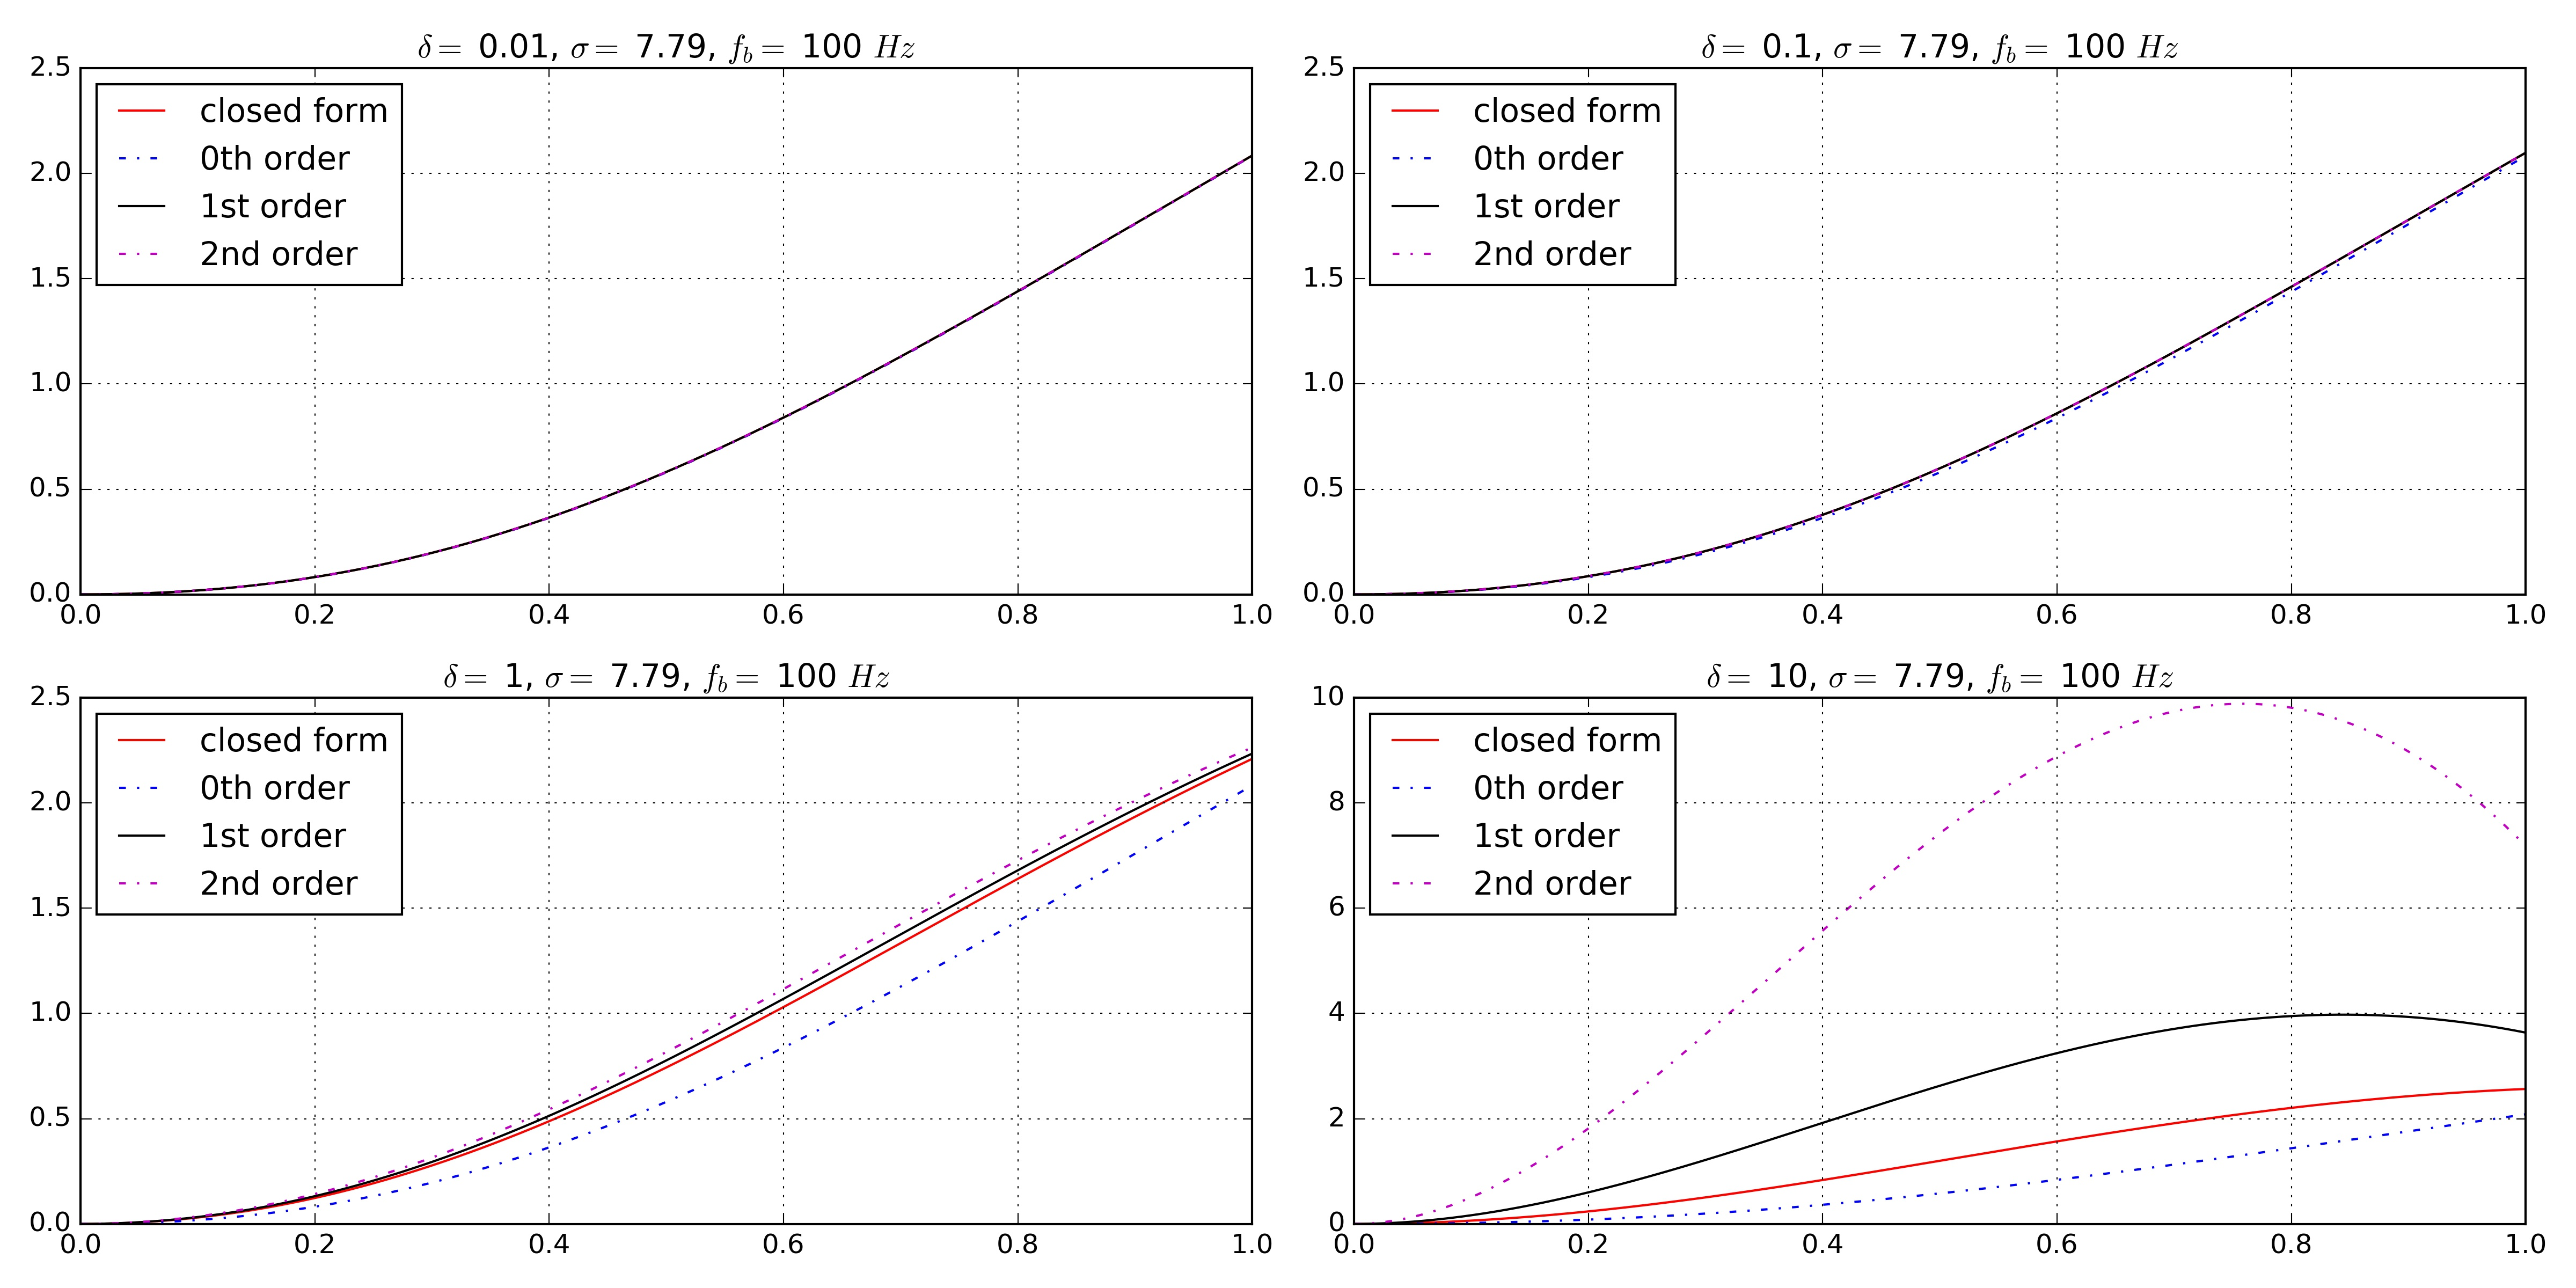
\includegraphics[width=\textwidth]{./img_eig_asy/fig_sol_analytic_disp_cmp_fr100}
    \caption{Comparison for the different orders of asymptotic expansion for the dimensionless relative displacement function $u_\delta(z)$.}
    \label{fig:fig_sol_analytic_disp_cmp_fr100}
\end{figure}


Theoretically, the first order derivative of the dimensionless relative displacement funtion $u(z;\delta)$ is 
\begin{equation}
    u^{\prime}(z;\delta) = \sigma^{1/2} \left( - A_\delta \sin{\sqrt{\sigma}z} + B_\delta \cos{\sqrt{\sigma}z} + C_\delta \sinh{\sqrt{\sigma}z} + D_\delta \cosh{\sqrt{\sigma}z} \right).
\end{equation}
\begin{equation}
    \chi_p = u_1^\prime(1) = \frac{ \sqrt{\sigma} \left( \sinh\sqrt{\sigma} - \sin\sqrt{\sigma} \right) }{ 1 + \cos\sqrt{\sigma } \cosh\sqrt{\sigma } + \frac{j \beta \sqrt{\sigma}}{ 1+ j \beta \sigma } \delta \left( \cos\sqrt{\sigma } \sinh\sqrt{\sigma } + \sin\sqrt{\sigma } \cosh\sqrt{\sigma } \right) }.
    \label{eq:eq_peh_perfs_compact_form_end_ders1}
\end{equation}
The value of this function at the free end ($z=1$) is just the output index $\chi_p$ according to equation (\ref{eq:eq_peh_perfs_compact_form_end_ders}). To see the influences of $\delta$ and $f_b$, therefore $\sigma$, upon $\chi_p$, we firslty calcualte the values of $\chi_p$ for different values of $\delta$ by fixing the value of $f_b$ to be some discrete values. The results are shown in Figure~\ref{fig:fig_sol_analytic_out_index_vs_delta}. 


\begin{figure}[!htbp]
    \centering
    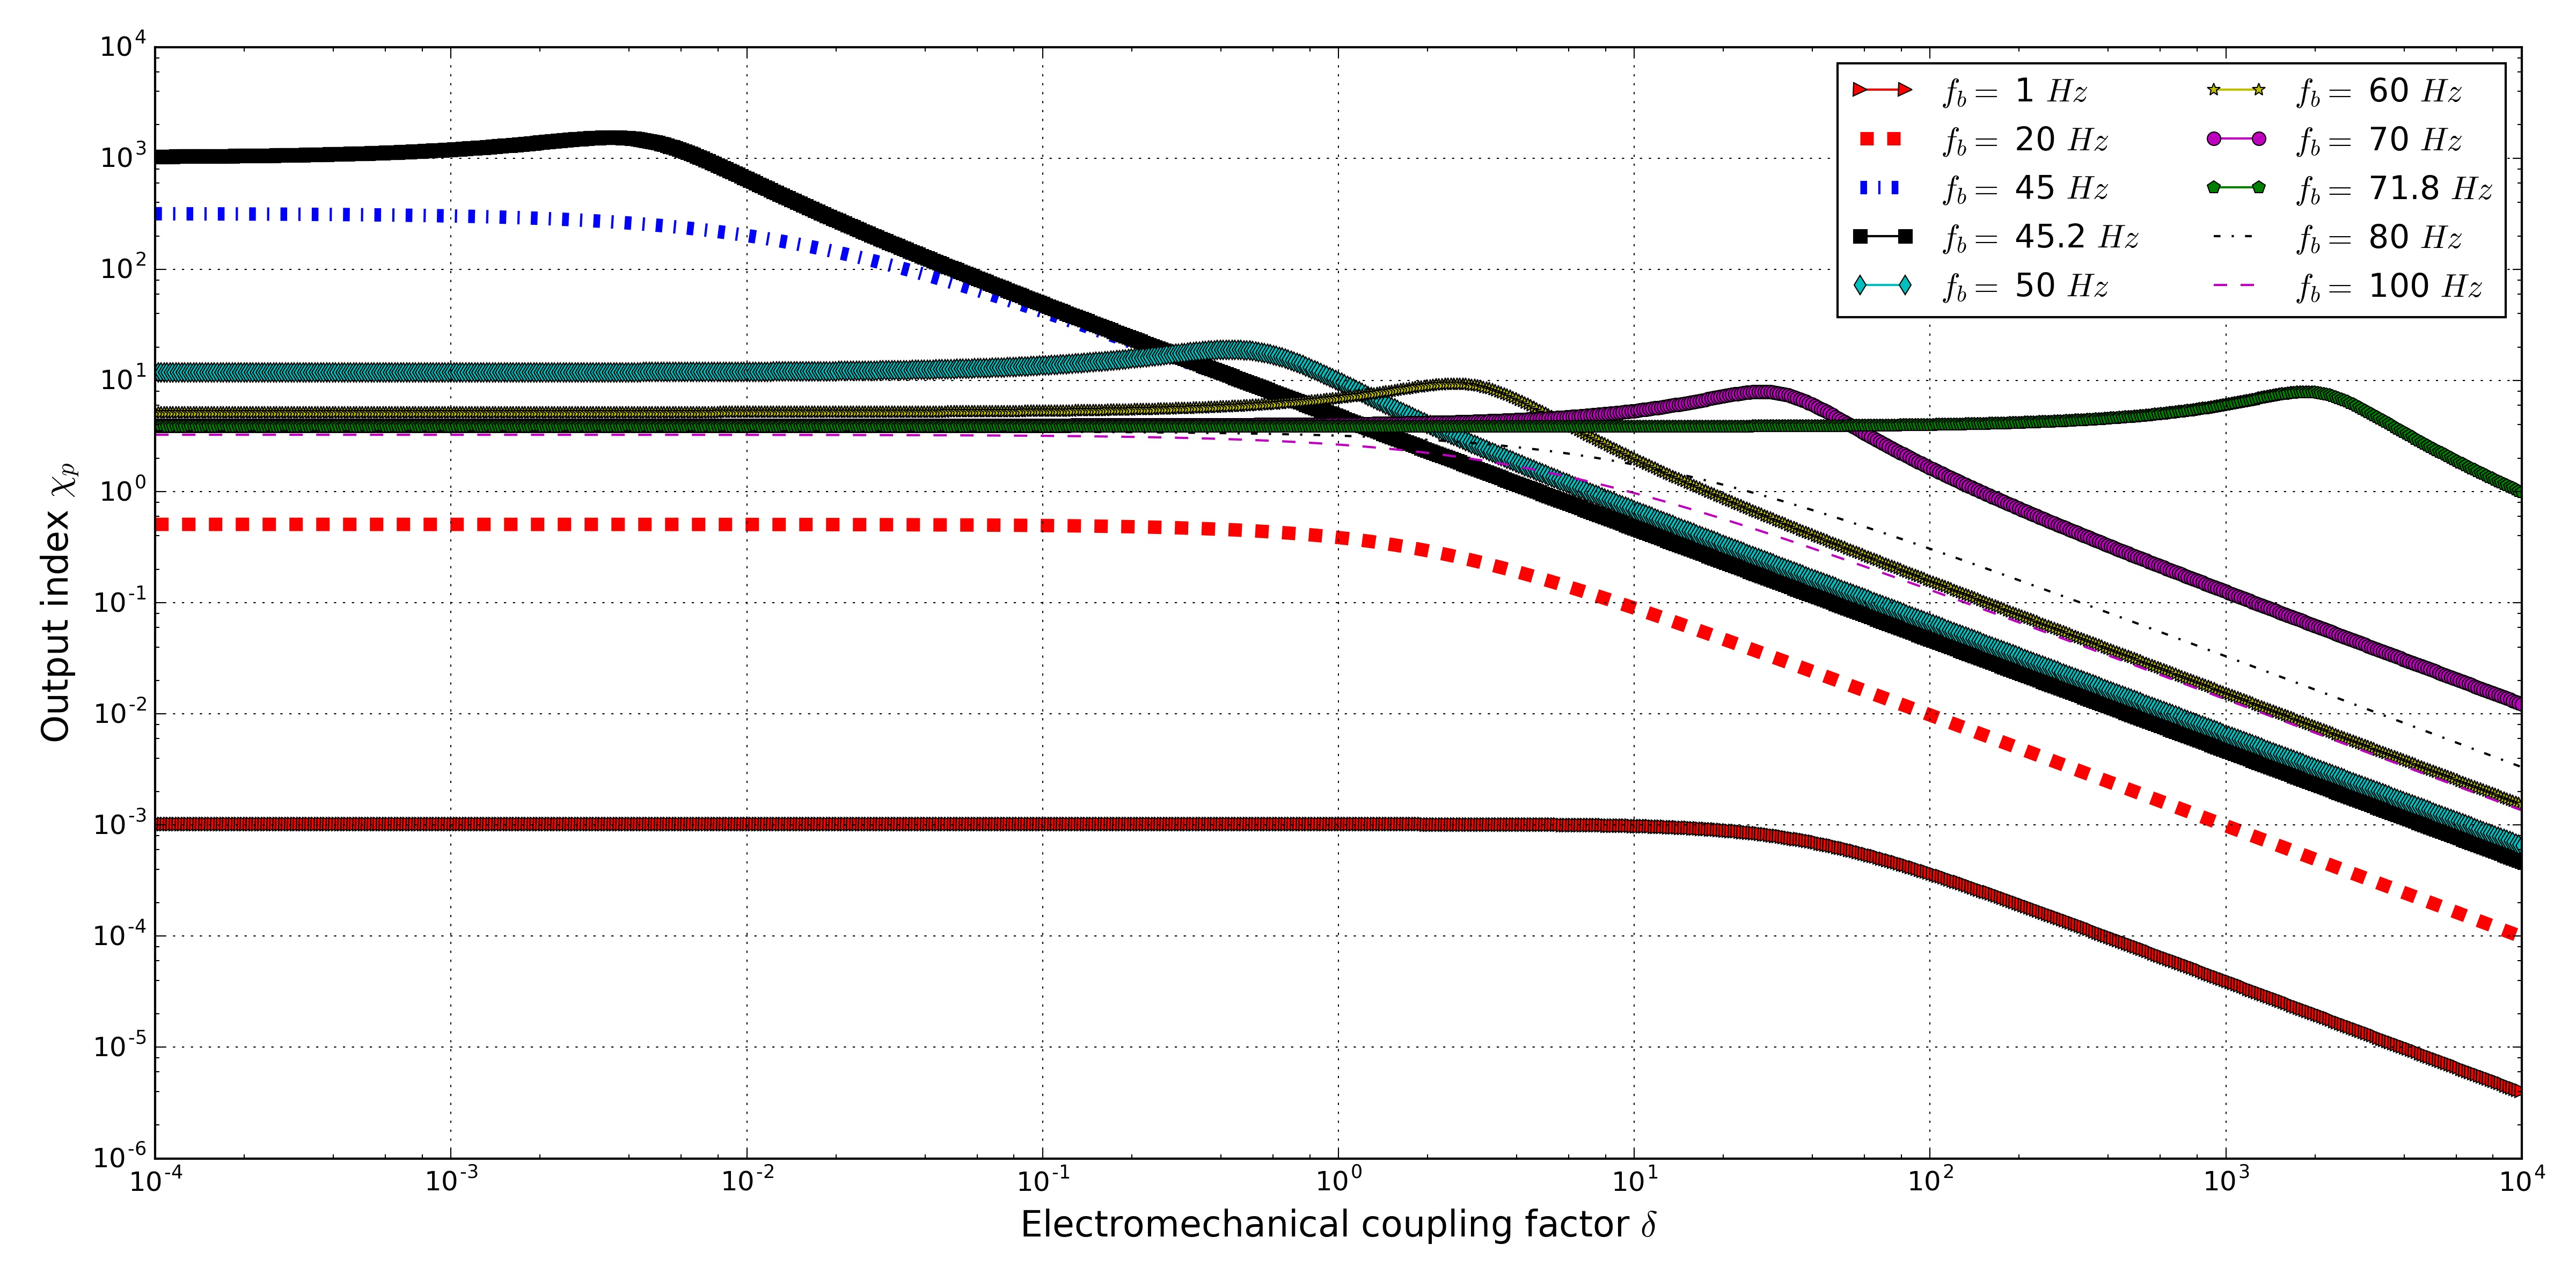
\includegraphics[width=\textwidth]{./img_eig_asy/fig_sol_analytic_out_index_vs_delta}
    \caption{Output index $\chi_p$ as a function of electromechanical coupling factor $\delta$ at different values of base excitation frequency $f_b$.}
    \label{fig:fig_sol_analytic_out_index_vs_delta}
\end{figure}


It is seen that the dependence of $\chi_p$ upon $\delta$ shows two different modes in the frequency range of $1\ - \ 100\ Hz$. For the frequencies of $45.2\ Hz \leq f_b \leq 71.8\ Hz$, a peak corresponding to a critical value of $\delta_p$ is present in the considered range of $\delta$. When $\delta$ is smaller than $\delta_p$, the output index $\chi_p$ increases along with $\delta$, and when $\delta$ is larger than $\delta_p$, the output index $\chi_p$ decreases with the increase of $\delta$. On the other hand, for the frequency range of $f_b \leq 45\ Hz$ or $f_b \geq 80\ Hz$, the output index $\chi_p$ shows a monotonical decrease with respect to the increase $\delta$.


\begin{figure}[!htbp]
    \centering
    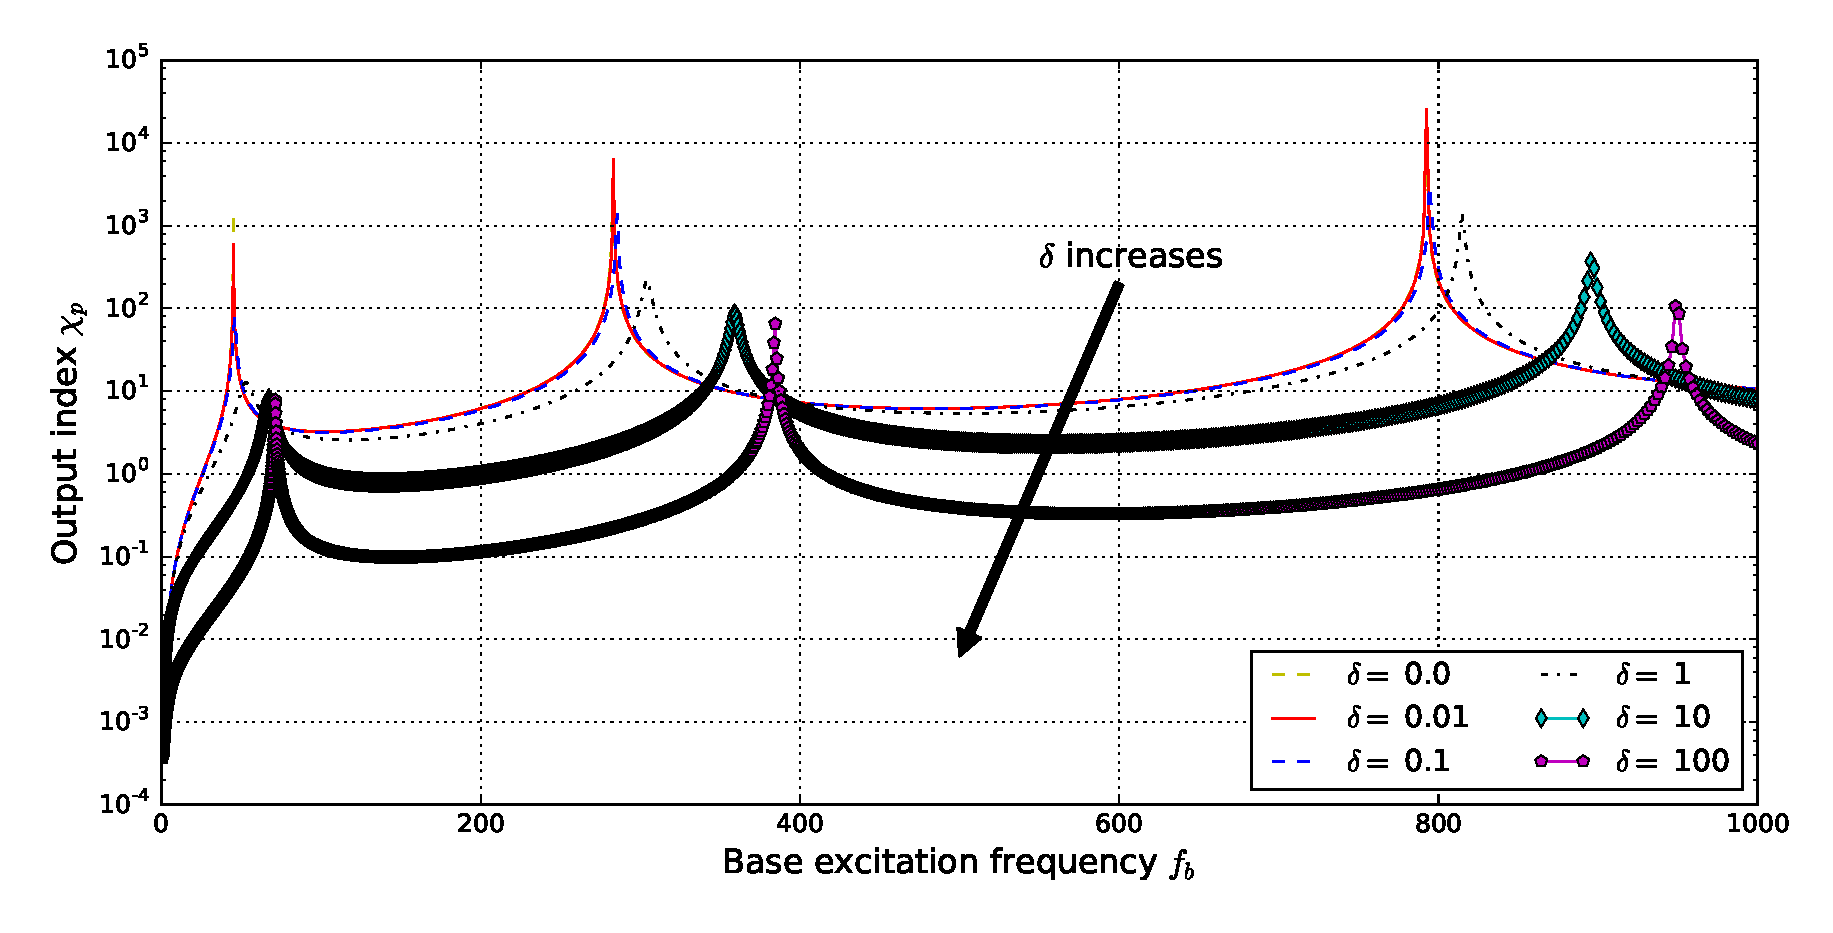
\includegraphics[width=\textwidth]{./img_eig_asy/fig_sol_analytic_out_index_vs_fr}
    \caption{Output index $\chi_p$ as a function of base excitation frequency $f_b$ at different values of electromechanical coupling factor $\delta$.}
    \label{fig:fig_sol_analytic_out_index_vs_fr}
\end{figure}


Alternatively, by fixing the values of $\delta$ to a discrete set of numbers, we calculate the values of $\chi_p$ in relation to different values of $f_b$. This is very similar to a frequency response of the output index as a function of $\sigma$. The results are shown in Figure~\ref{fig:fig_sol_analytic_out_index_vs_fr}. It is clearly shown that with the increase of electromechanical coupling factor $\delta$, the resonant frequencies to the system increase with the increase of $\delta$. This is clearly shown in the shift to the right of the frequency response curve. Besides, we add in this figure the case where $\delta = 0.0$ as a reference. Simple comparisons show that the discrepency between the frequency response curves related to the case of $\delta = 0$, $\delta=0.01$, and $\delta = 0.1$ is small. A direct conclusion is that for relatively small values of electromechanical coupling factor $\delta$, the output index $\chi_p$ can be approximated by 
\begin{equation}
    \chi_p \approx \frac{ \sqrt{\sigma} \left( \sinh\sqrt{\sigma} - \sin\sqrt{\sigma} \right) }{ 1 + \cos\sqrt{\sigma } \cosh\sqrt{\sigma } }.
\end{equation}

As a result, the output performance measures $\tilde{V}_p$, $\tilde{I}_p$, and $\tilde{P}_p$ can be approximated by 
\begin{equation}
    \left\{\begin{aligned}
        \tilde{V}_p &= - \frac{j \sigma \beta}{j \sigma \beta + 1} \left(\frac{\eta_b}{l_p}\right) \left(\frac{e_p}{C_p}\right) \chi_p , \\
        &= - \frac{j \sigma \beta}{j \sigma \beta + 1} \left(\frac{\eta_b}{l_p}\right) \left(\frac{e_p}{C_p}\right) \frac{ \sqrt{\sigma} \left( \sinh\sqrt{\sigma} - \sin\sqrt{\sigma} \right) }{ 1 + \cos\sqrt{\sigma } \cosh\sqrt{\sigma } } , \\
        \tilde{I}_p &=  \tilde{V}_p / R_l = - \frac{ j \sigma \beta } {j \sigma \beta + 1} \left( \frac{\eta_b}{l_p} \right) \left( \frac{e_p}{C_p R_l} \right) \chi_p , \\
        &= - \frac{ j \sigma \beta } {j \sigma \beta + 1} \left( \frac{\eta_b}{l_p} \right) \left( \frac{e_p}{C_p R_l} \right) \frac{ \sqrt{\sigma} \left( \sinh\sqrt{\sigma} - \sin\sqrt{\sigma} \right) }{ 1 + \cos\sqrt{\sigma } \cosh\sqrt{\sigma } }, \\
        \tilde{P}_p &=  \tilde{V}_p^2 / R_l = \left(\frac{\eta_b}{l_p}\right)^2 \left(\frac{e_p}{C_p}\right) \left( \frac{e_p}{C_p R_l} \right) \left( \frac{ j \sigma \beta}{ j \sigma \beta + 1 } \right)^2 \chi_p^2, \\
        &= \left(\frac{\eta_b}{l_p}\right)^2 \left(\frac{e_p}{C_p}\right) \left( \frac{e_p}{C_p R_l} \right) \left( \frac{ j \sigma \beta}{ j \sigma \beta + 1 } \right)^2 \left( \frac{ \sqrt{\sigma} \left( \sinh\sqrt{\sigma} - \sin\sqrt{\sigma} \right) }{ 1 + \cos\sqrt{\sigma } \cosh\sqrt{\sigma } } \right)^2.
    \end{aligned}\right.
    \label{eq:eq_peh_perfs_compact_form_approx}
\end{equation}


\begin{figure}[!htbp]
    \centering
    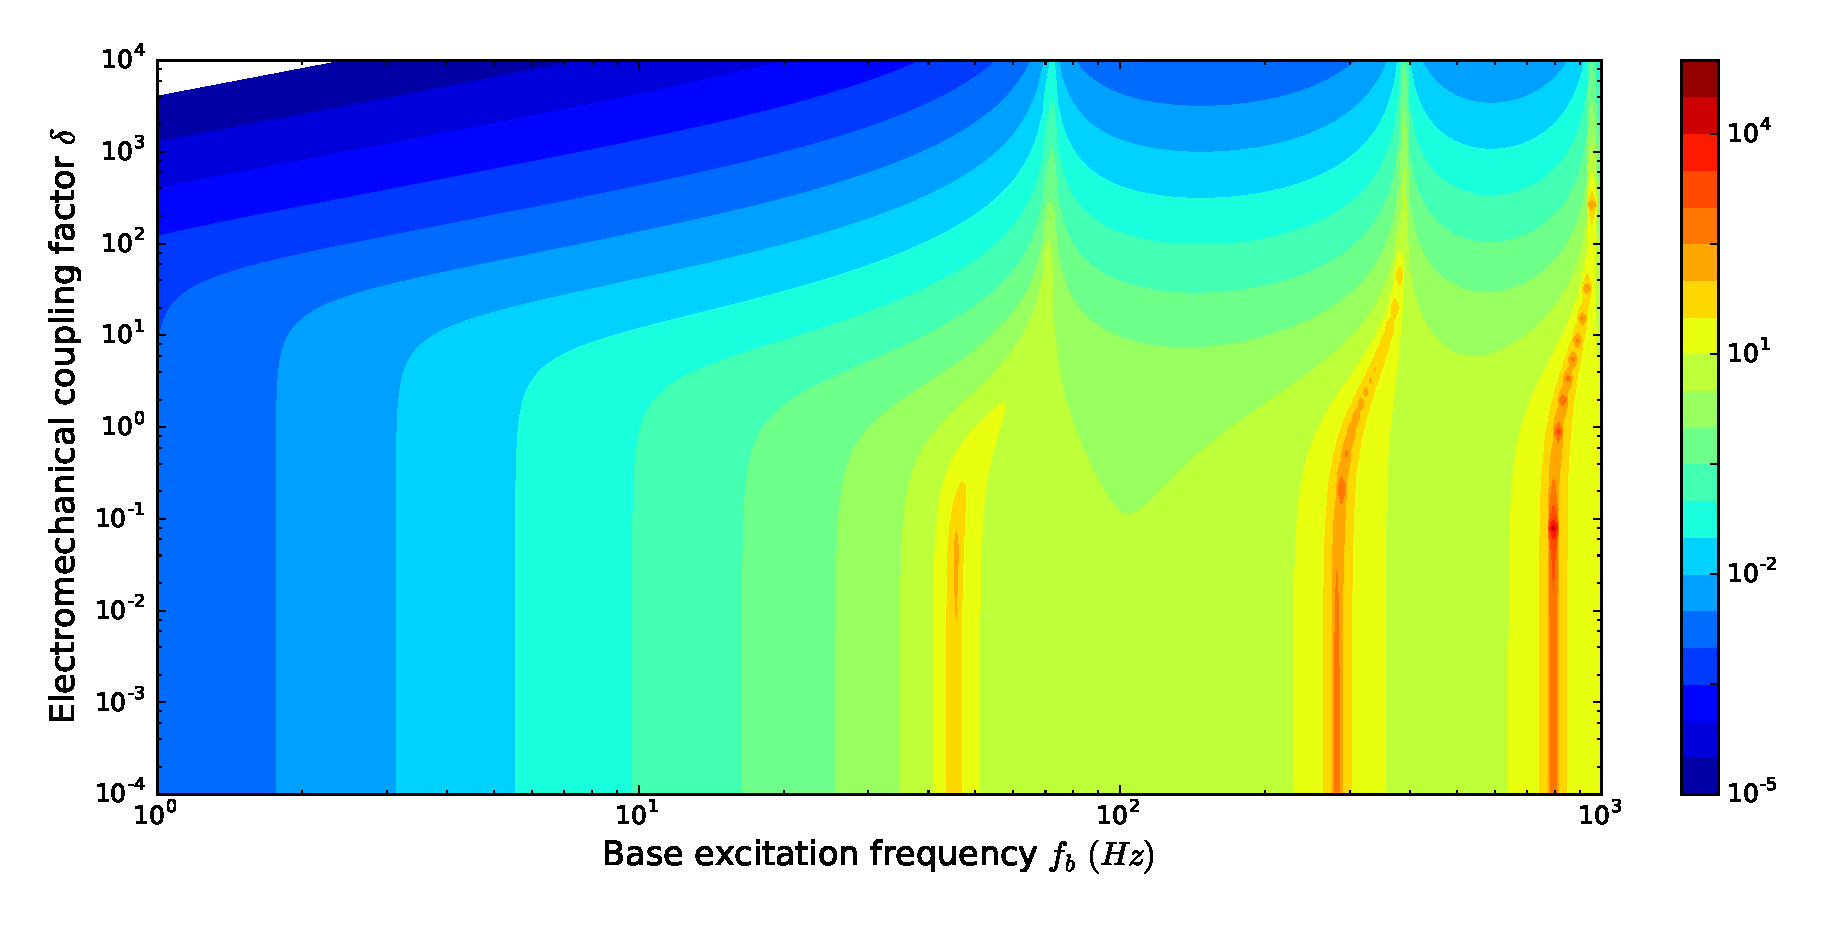
\includegraphics[width=\textwidth]{./img_eig_asy/fig_sol_analytic_out_index_contour}
    \caption{Output index $\chi_p$ as a function of base excitation frequency $f_b$ and electromechanical coupling factor $\delta$.}
    \label{fig:fig_sol_analytic_out_index_contour}
\end{figure}



\begin{figure}[!htbp]
    \centering
    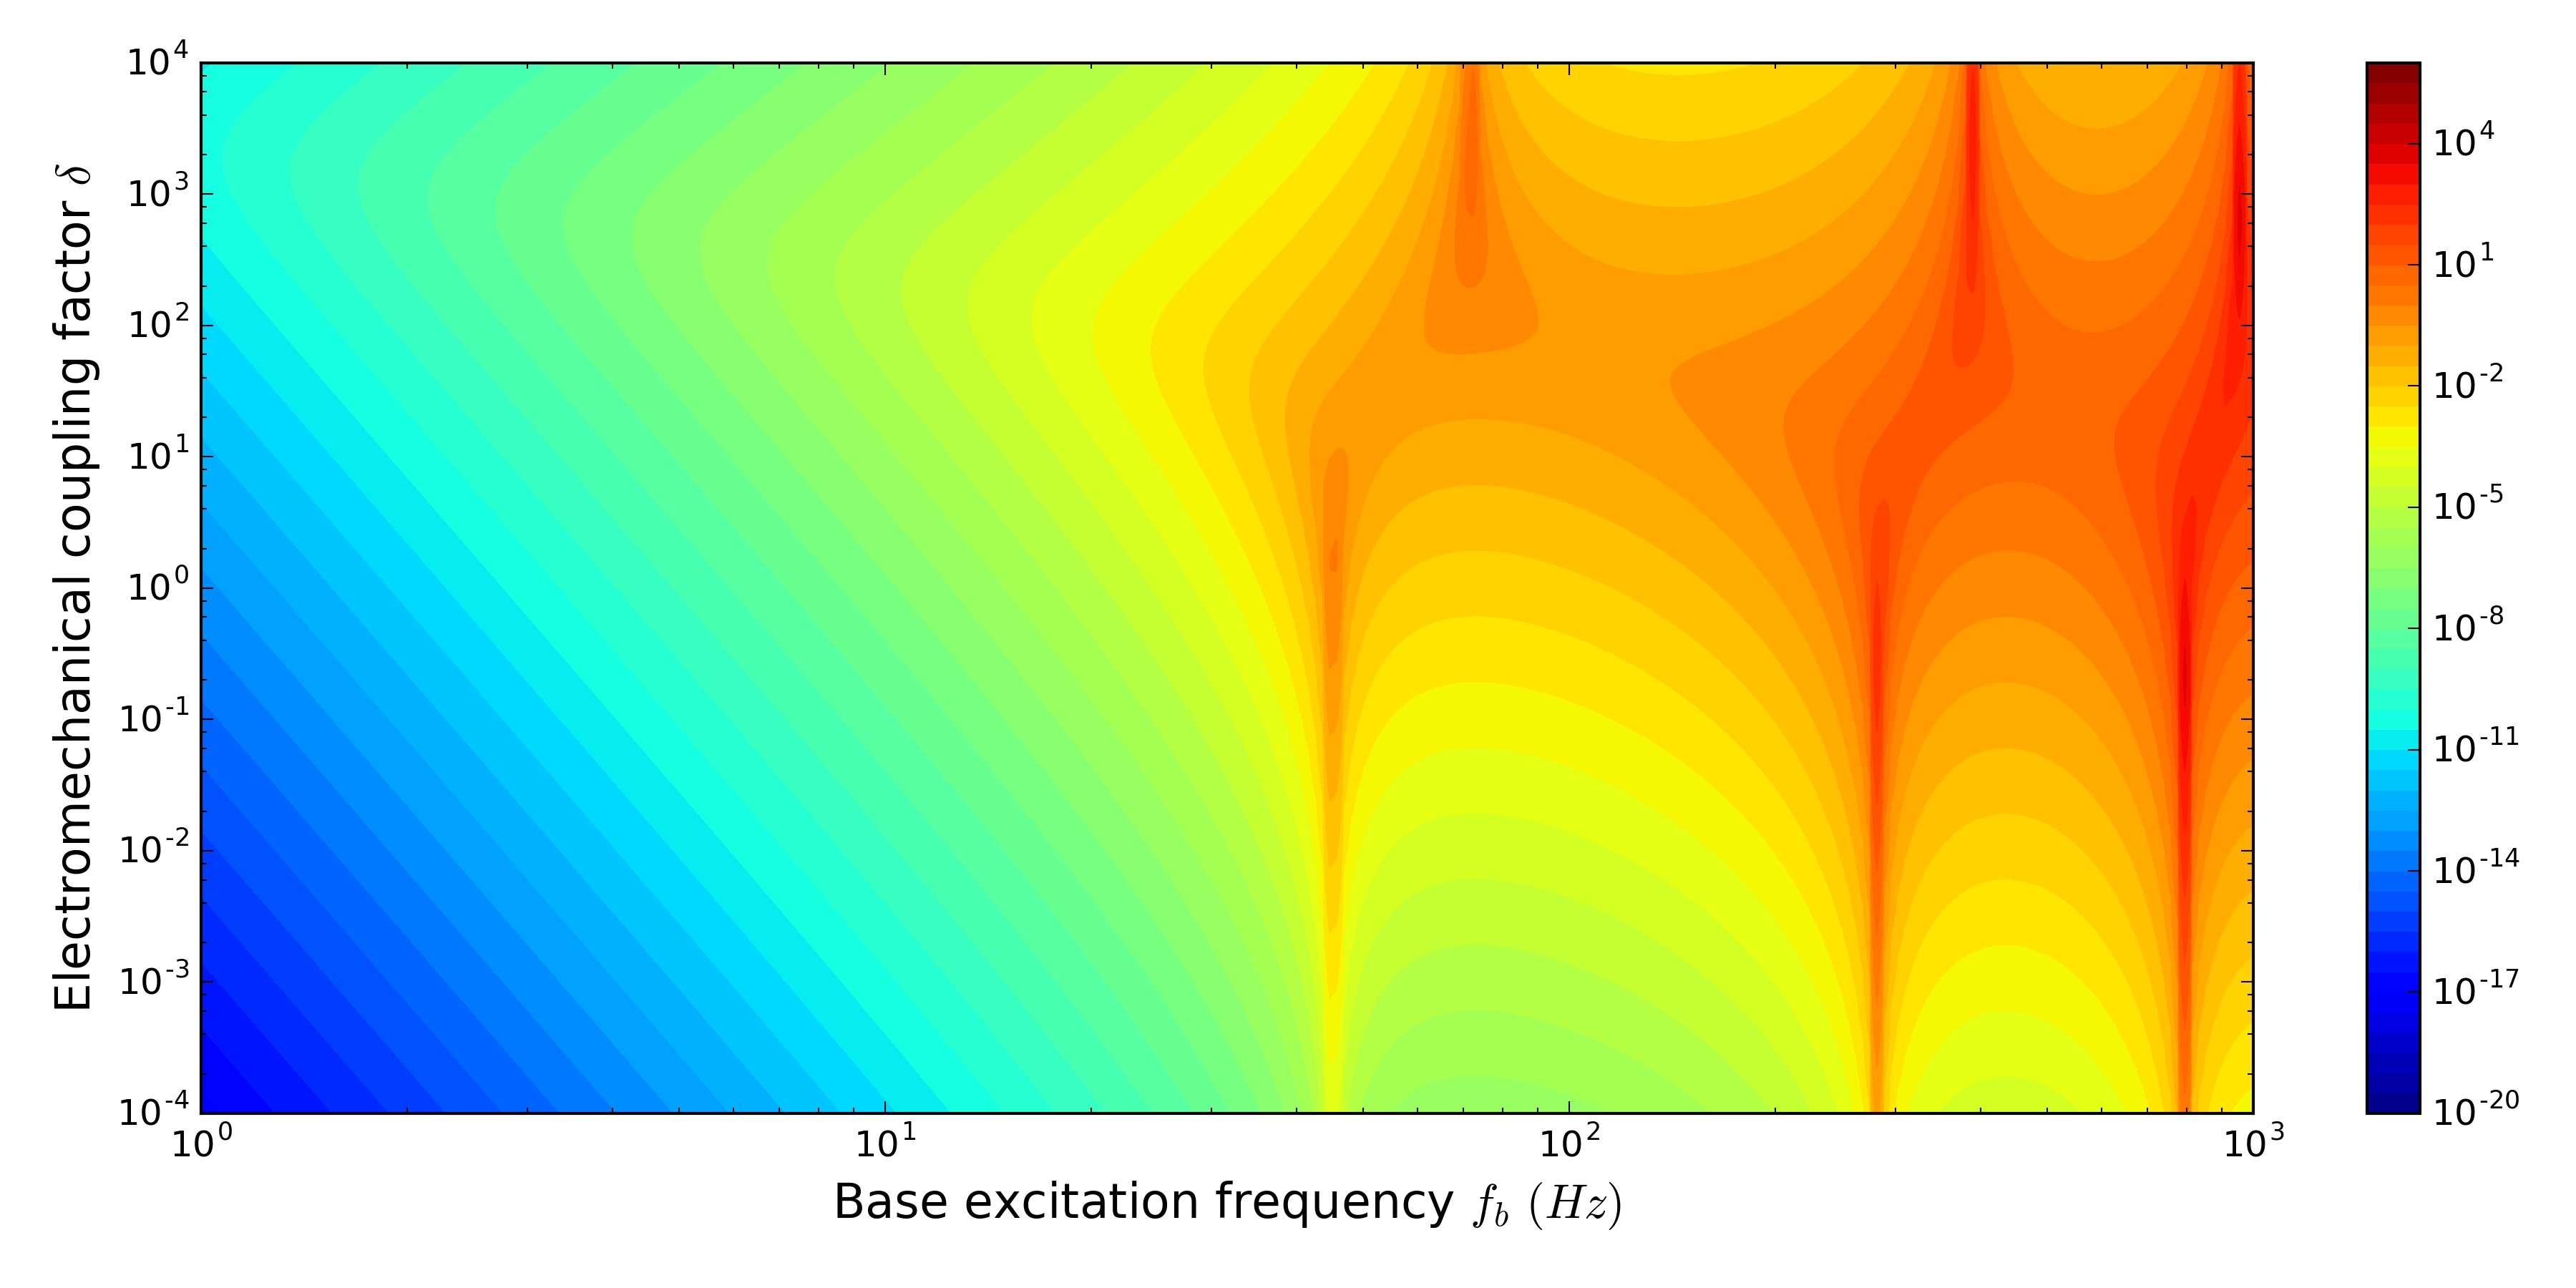
\includegraphics[width=\textwidth]{./img_eig_asy/fig_sol_analytic_out_vol_contour}
    \caption{Output voltage $\tilde{V}_p$ as a function of base excitation frequency $f_b$ and electromechanical coupling factor $\delta$.}
    \label{fig:fig_sol_analytic_out_vol_contour}
\end{figure}




\begin{figure}[!htbp]
    \centering
    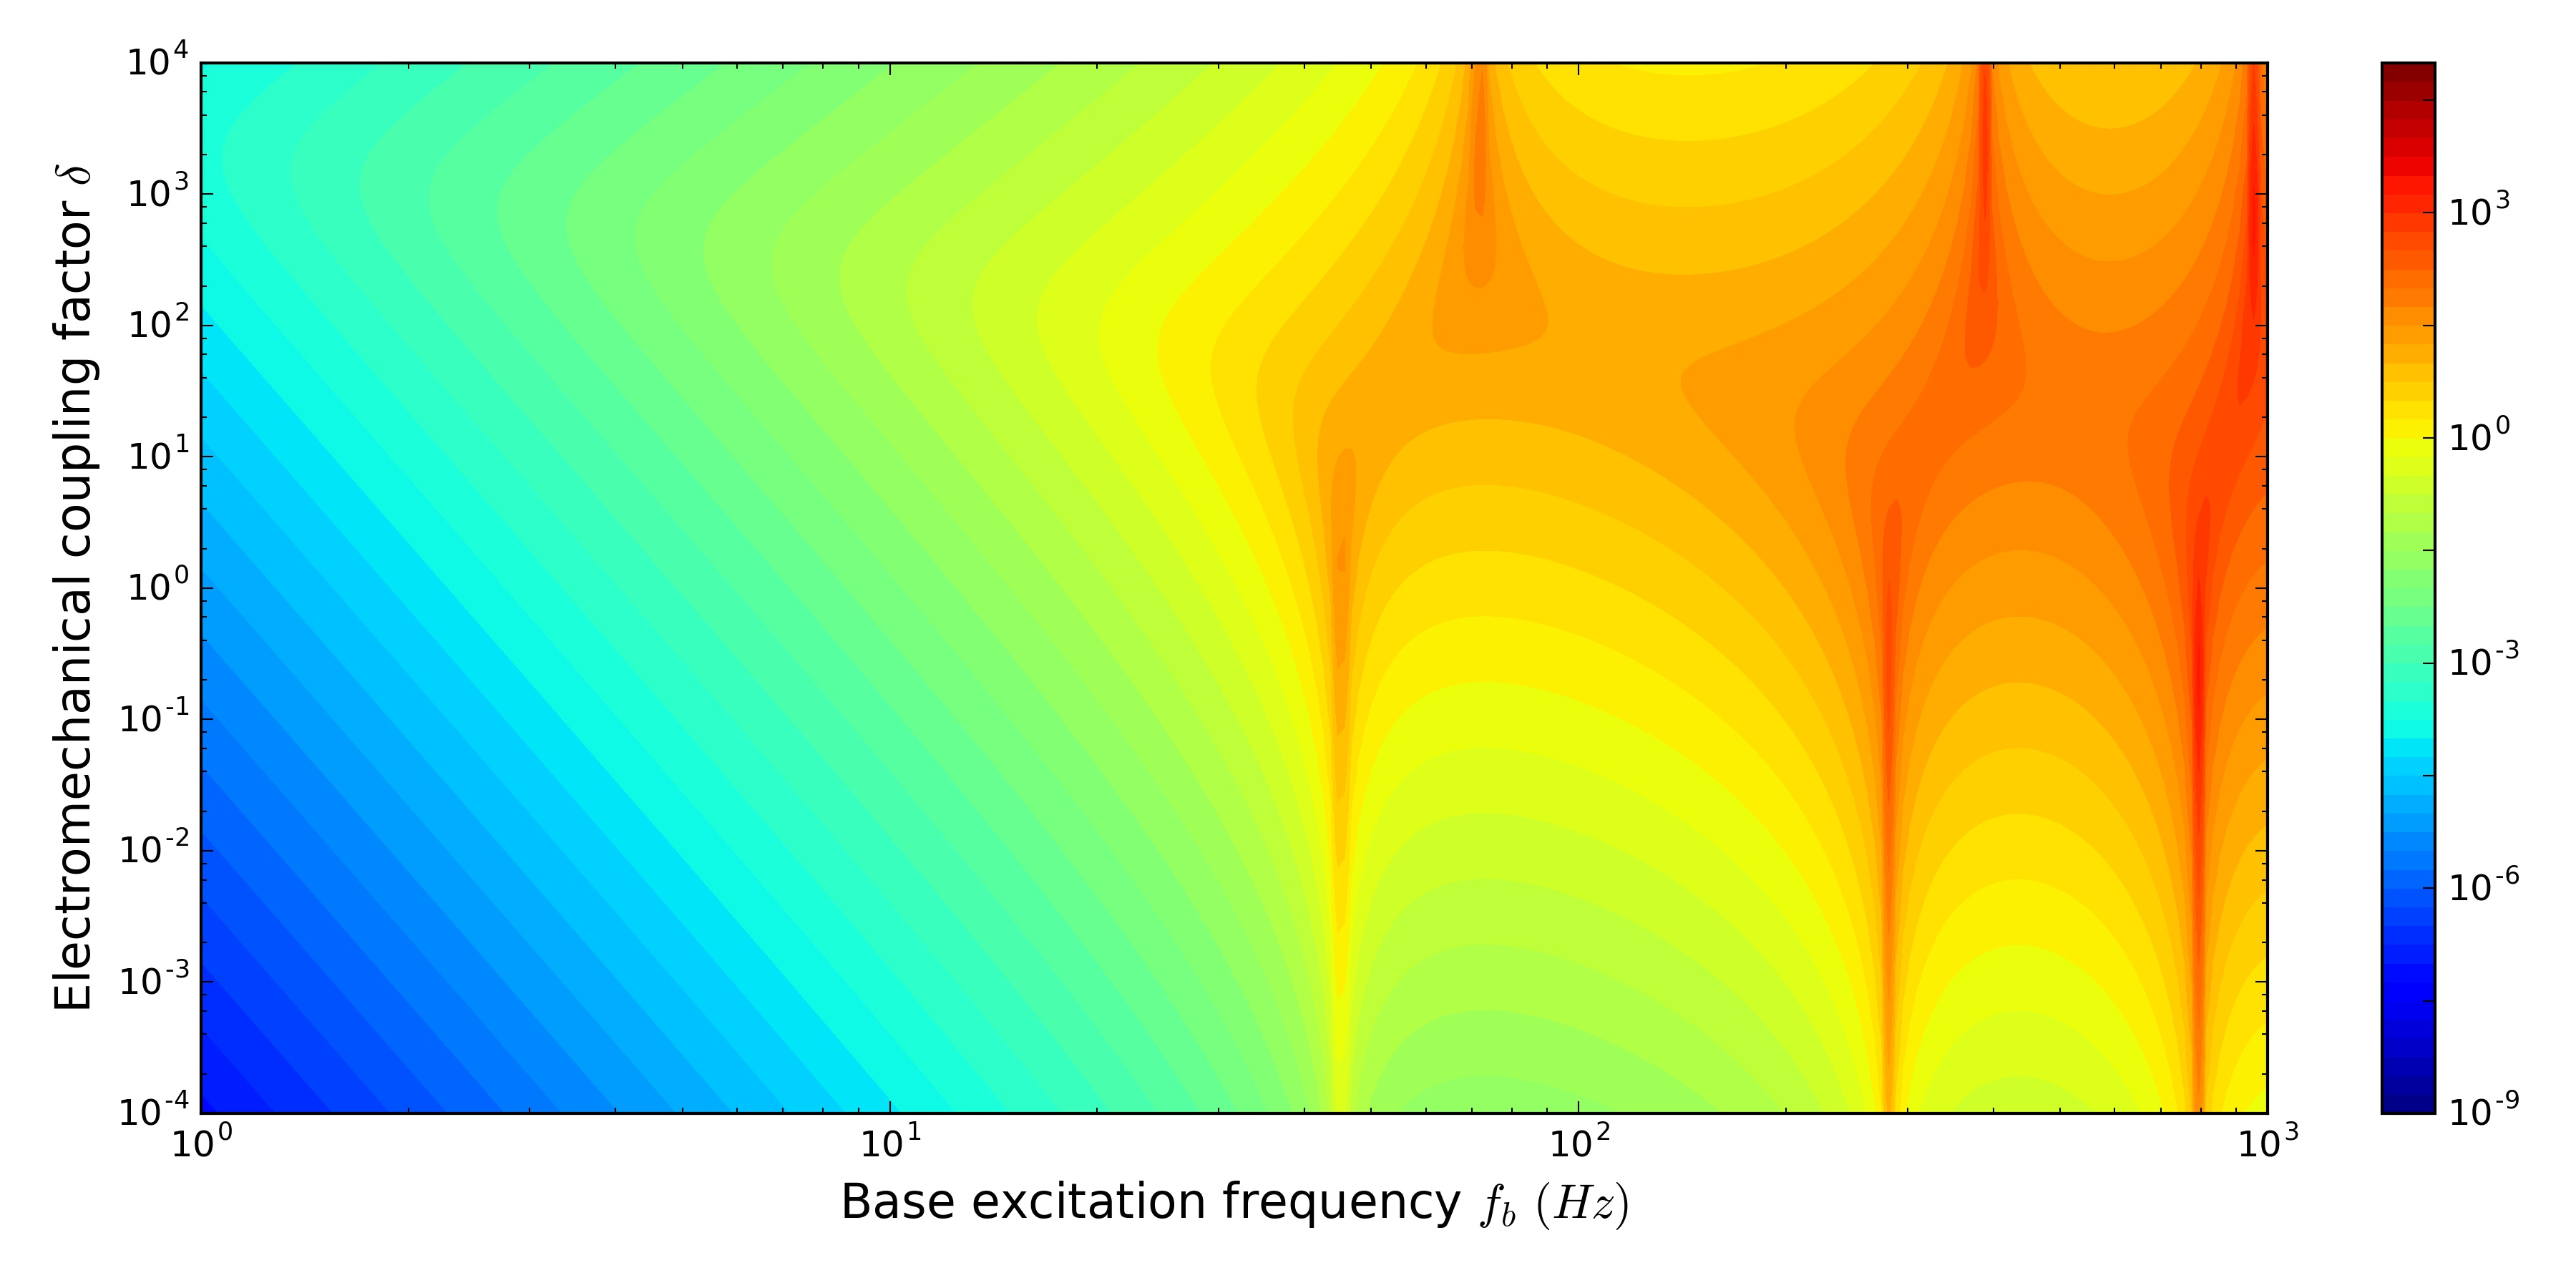
\includegraphics[width=\textwidth]{./img_eig_asy/fig_sol_analytic_out_pow_contour}
    \caption{Output voltage $\tilde{P}_p$ as a function of base excitation frequency $f_b$ and electromechanical coupling factor $\delta$.}
    \label{fig:fig_sol_analytic_out_pow_contour}
\end{figure}










\section{Conclusion}



















\section*{Appendices}

The asymptotic expansion of equation (\ref{eq:eq_disp_func_coeffs_exps}) can be found using an iterative method. In fact, for higher order expansions ($k \geq 1$), we have the following iterative relation: 
\begin{equation}
    \left\{\begin{aligned}
        A_{k+1} + C_{k+1} &= 0, \\
        B_{k+1} + D_{k+1} &= 0, \\
        \left( - A_{k+1} \cos{\sqrt{\sigma}} - B_{k+1} \sin{\sqrt{\sigma}} + C_{k+1} \cosh{\sqrt{\sigma}} + D_{k+1} \sinh{\sqrt{\sigma}} \right) &+ \\
        \frac{j \beta \sqrt{\sigma}}{ j\sigma \beta + 1 } \left( - A_{k} \sin{\sqrt{\sigma}} + B_{k} \cos{\sqrt{\sigma}} + C_{k} \sinh{\sqrt{\sigma}} + D_{k} \cosh{\sqrt{\sigma}} \right) &= 0, \\
        A_{k+1} \sin{\sqrt{\sigma}} - B_{k+1} \cos{\sqrt{\sigma}} + C_{k+1} \sinh{\sqrt{\sigma}} + D_{k+1} \cosh{\sqrt{\sigma}} &= 0,
    \end{aligned}\right.
\end{equation}
whose solution is expressed by
\begin{equation}
    \left\{\begin{aligned}
        A_{k+1} &= \left( \frac{j \beta \sqrt{\sigma }}{1+j \beta \sigma } \right) \left(\frac{\cos\sqrt{\sigma }+\cosh\sqrt{\sigma }}{2 \cos\sqrt{\sigma }\cosh\sqrt{\sigma }+2} \right) \left( Q_k \right), \\
        B_{k+1} &= \left( \frac{j \beta \sqrt{\sigma }}{1+j \beta \sigma } \right) \left( \frac{-\sinh\sqrt{\sigma }+\sin\sqrt{\sigma }}{2 \cos\sqrt{\sigma }\cosh\sqrt{\sigma }+2} \right) \left( Q_k \right), \\
        C_{k+1} &= \left( \frac{j \beta \sqrt{\sigma }}{1+j \beta \sigma } \right) \left( -\frac{\cos\sqrt{\sigma }+\cosh\sqrt{\sigma }}{2 \cos\sqrt{\sigma } \cosh\sqrt{\sigma }+2} \right) \left( Q_k \right), \\
        D_{k+1} &= \left( \frac{j \beta \sqrt{\sigma }}{1+j \beta \sigma } \right) \left( \frac{-\sin\sqrt{\sigma }+\sinh\sqrt{\sigma }}{2 \cos\sqrt{\sigma }\cosh\sqrt{\sigma }+2} \right) \left( Q_k \right), 
    \end{aligned}\right.
\end{equation}
in which
\begin{equation}
    Q_k = - A_{k} \sin{\sqrt{\sigma}} + B_{k} \cos{\sqrt{\sigma}} + C_{k} \sinh{\sqrt{\sigma}} + D_{k} \cosh{\sqrt{\sigma}}.
\end{equation}


In terms of $Q_k$ ($k \geq 0$), we have the following iterative relation
% \begin{equation}
%     \begin{aligned}
%         Q_{k+1} &= - A_{k+1} \sin{\sqrt{\sigma}} + B_{k+1} \cos{\sqrt{\sigma}} + C_{k+1} \sinh{\sqrt{\sigma}} + D_{k+1} \cosh{\sqrt{\sigma}} \\
%         &= - \left( \frac{ \sin\sqrt{\sigma} \cosh\sqrt{\sigma} + \cos\sqrt{\sigma} \sinh\sqrt{\sigma} }{ \cos\sqrt{\sigma }\cosh\sqrt{\sigma }+1 } \right) \left( \frac{j \beta \sqrt{\sigma }}{1+j \beta \sigma } \right) Q_k,
%     \end{aligned}
% \end{equation}
\begin{equation}
    Q_{k+1} = - \left( \frac{ \sin\sqrt{\sigma} \cosh\sqrt{\sigma} + \cos\sqrt{\sigma} \sinh\sqrt{\sigma} }{ \cos\sqrt{\sigma }\cosh\sqrt{\sigma }+1 } \right) \left( \frac{j \beta \sqrt{\sigma }}{1+j \beta \sigma } \right) Q_k,
\end{equation}
and the initial two values $Q_0$ and $Q_1$:
% \begin{equation}
%     \begin{aligned}
%         Q_{1} &= - A_1 \sin{\sqrt{\sigma}} + B_1 \cos{\sqrt{\sigma}} + C_1 \sinh{\sqrt{\sigma}} + D_1 \cosh{\sqrt{\sigma}} \\
%         &= \frac{j \beta  \sqrt{\sigma }}{1+j \beta  \sigma } \left(\frac{\sin\sqrt{\sigma } -\sinh\sqrt{\sigma }}{\cos\sqrt{\sigma } \cosh\sqrt{\sigma }+1} \right)  \left( \frac{\cos\sqrt{\sigma } \sinh\sqrt{\sigma }+\sin\sqrt{\sigma } \cosh\sqrt{\sigma }}{\cos\sqrt{\sigma } \cosh\sqrt{\sigma }+1} \right)
%     \end{aligned}
% \end{equation}
% \begin{equation}
%     Q_0 = \frac{\sinh\sqrt{\sigma }-\sin\sqrt{\sigma }}{\cos\sqrt{\sigma } \cosh\sqrt{\sigma }+1}
% \end{equation}
\begin{equation}
    \left\{\begin{aligned}
        Q_0 &= \frac{\sinh\sqrt{\sigma }-\sin\sqrt{\sigma }}{\cos\sqrt{\sigma } \cosh\sqrt{\sigma }+1}, \\
        Q_{1} &= \frac{j \beta  \sqrt{\sigma }}{1+j \beta  \sigma } \left(\frac{\sin\sqrt{\sigma } -\sinh\sqrt{\sigma }}{\cos\sqrt{\sigma } \cosh\sqrt{\sigma }+1} \right)  \left( \frac{\cos\sqrt{\sigma } \sinh\sqrt{\sigma }+\sin\sqrt{\sigma } \cosh\sqrt{\sigma }}{\cos\sqrt{\sigma } \cosh\sqrt{\sigma }+1} \right).
    \end{aligned}\right.
\end{equation}
Hence it is shown that for $k \geq 0$,
% \begin{equation}
%     \begin{aligned}
%         Q_{k} &= - \left( \frac{ \sin\sqrt{\sigma} \cosh\sqrt{\sigma} + \cos\sqrt{\sigma} \sinh\sqrt{\sigma} }{ \cos\sqrt{\sigma }\cosh\sqrt{\sigma }+1 } \right) \left( \frac{j \beta \sqrt{\sigma }}{1+j \beta \sigma } \right) Q_k \\
%         &= \left[- \left( \frac{j \beta \sqrt{\sigma }}{1+j \beta \sigma } \right) \left( \frac{ \sin\sqrt{\sigma} \cosh\sqrt{\sigma} + \cos\sqrt{\sigma} \sinh\sqrt{\sigma} }{ \cos\sqrt{\sigma }\cosh\sqrt{\sigma }+1 } \right)  \right]^k \left( \frac{\sinh\sqrt{\sigma }-\sin\sqrt{\sigma }}{\cos\sqrt{\sigma } \cosh\sqrt{\sigma }+1} \right)
%     \end{aligned}
% \end{equation}
\begin{equation}
    Q_{k} = \left[- \left( \frac{j \beta \sqrt{\sigma }}{1+j \beta \sigma } \right) \left( \frac{ \sin\sqrt{\sigma} \cosh\sqrt{\sigma} + \cos\sqrt{\sigma} \sinh\sqrt{\sigma} }{ \cos\sqrt{\sigma }\cosh\sqrt{\sigma }+1 } \right)  \right]^k \left( \frac{\sinh\sqrt{\sigma }-\sin\sqrt{\sigma }}{\cos\sqrt{\sigma } \cosh\sqrt{\sigma }+1} \right).
\end{equation}
As a result, we obtain that for $k \geq 1$,
\footnotesize
\begin{equation*}
    \left\{\begin{aligned}
        A_{k} &= \left( \frac{j \beta \sqrt{\sigma }}{1+j \beta \sigma } \right)^{k} \left( \frac{ -\sin\sqrt{\sigma} \cosh\sqrt{\sigma} - \cos\sqrt{\sigma} \sinh\sqrt{\sigma} }{ \cos\sqrt{\sigma }\cosh\sqrt{\sigma }+1 } \right)^{k-1} \left( \frac{\sinh\sqrt{\sigma }-\sin\sqrt{\sigma }}{\cos\sqrt{\sigma } \cosh\sqrt{\sigma }+1} \right) \left(\frac{\cos\sqrt{\sigma }+\cosh\sqrt{\sigma }}{2 \cos\sqrt{\sigma }\cosh\sqrt{\sigma }+2} \right), \\
        B_{k} &= \left( \frac{j \beta \sqrt{\sigma }}{1+j \beta \sigma } \right)^{k}  \left( \frac{ -\sin\sqrt{\sigma} \cosh\sqrt{\sigma} - \cos\sqrt{\sigma} \sinh\sqrt{\sigma} }{ \cos\sqrt{\sigma }\cosh\sqrt{\sigma }+1 } \right)^{k-1} \left( \frac{\sinh\sqrt{\sigma }-\sin\sqrt{\sigma }}{\cos\sqrt{\sigma } \cosh\sqrt{\sigma }+1} \right) \left( \frac{-\sinh\sqrt{\sigma }+\sin\sqrt{\sigma }}{2 \cos\sqrt{\sigma }\cosh\sqrt{\sigma }+2} \right), \\
        C_{k} &= \left( \frac{j \beta \sqrt{\sigma }}{1+j \beta \sigma } \right)^{k}  \left( \frac{ -\sin\sqrt{\sigma} \cosh\sqrt{\sigma} - \cos\sqrt{\sigma} \sinh\sqrt{\sigma} }{ \cos\sqrt{\sigma }\cosh\sqrt{\sigma }+1 } \right)^{k-1} \left( \frac{\sinh\sqrt{\sigma }-\sin\sqrt{\sigma }}{\cos\sqrt{\sigma } \cosh\sqrt{\sigma }+1} \right) \left( \frac{-\cos\sqrt{\sigma }-\cosh\sqrt{\sigma }}{2 \cos\sqrt{\sigma } \cosh\sqrt{\sigma }+2} \right), \\
        D_{k} &= \left( \frac{j \beta \sqrt{\sigma }}{1+j \beta \sigma } \right)^{k} \left( \frac{ -\sin\sqrt{\sigma} \cosh\sqrt{\sigma} - \cos\sqrt{\sigma} \sinh\sqrt{\sigma} }{ \cos\sqrt{\sigma }\cosh\sqrt{\sigma }+1 } \right)^{k-1} \left( \frac{\sinh\sqrt{\sigma }-\sin\sqrt{\sigma }}{\cos\sqrt{\sigma } \cosh\sqrt{\sigma }+1} \right) \left( \frac{-\sin\sqrt{\sigma }+\sinh\sqrt{\sigma }}{2 \cos\sqrt{\sigma }\cosh\sqrt{\sigma }+2} \right).
    \end{aligned}\right.
\end{equation*}
\normalsize



\section*{Acknowledgements}


\bibliography{analysis_eig_asy.bib}
\bibliographystyle{vancouver}

\end{document}